\documentclass[12pt,a4paper,openright,twoside]{book}
\usepackage[utf8]{inputenc}
\usepackage{disi-thesis}
\usepackage{code-lstlistings}
\usepackage{notes}
\usepackage{shortcuts}
\usepackage{acronym}
\usepackage{caption}
\usepackage{subcaption}

\school{\unibo}
\programme{MSc in Engineering and Computer Science}
\title{Feasibility of Reactive Aggregate Programming via Kotlin Flows}
\author{Filippo Vissani}
\date{\today}
\subject{Laboratory of Software Systems}
\supervisor{Prof. Danilo Pianini}
\cosupervisor{Dott. Gianluca Aguzzi}
\session{IV}
\academicyear{2022-2023}

% Definition of acronyms
\acrodef{IoT}{Internet of Thing}
\acrodef{vm}[VM]{Virtual Machine}
\acrodef{jvm}[JVM]{Java Virtual Machine}
\acrodef{cas}[CAS]{Collective Adaptive Systems}
\acrodef{fc}[FC]{Field Calculus}

\mainlinespacing{1.241}

\begin{document}

\frontmatter\frontispiece

\begin{abstract}	
% Max 2000 characters, strict.
% Very brief (e.g. 250-300 words)
% Abstract should briefly point out: Context, Problem/Objectives, Methods/Contribution, Results, Conclusions
\end{abstract}

\begin{dedication} % this is optional
Optional. Max a few lines.
\end{dedication}

\begin{acknowledgements} % this is optional
Optional. Max 1 page.
\end{acknowledgements}

%----------------------------------------------------------------------------------------
\tableofcontents
\listoffigures     % (optional) comment if empty
\lstlistoflistings % (optional) comment if empty
%----------------------------------------------------------------------------------------

\mainmatter

%! Author = Filippo Vissani
%! Date = 08/02/24
% !TeX root = ../thesis-main.tex

%----------------------------------------------------------------------------------------
\chapter{Introduction}
\label{chap:introduction}
%----------------------------------------------------------------------------------------

Developing \textit{artificial self-organizing systems} with \textit{collective intelligence} poses a significant research challenge that spans multiple disciplines in science and engineering~\cite{Parunak2015, Gershenson2007, Singh2013, DeNicola2020}. A central problem involves guiding the \textit{self-organizing behavior among a group of agents or devices}, a task often referred to as "guided self-organization"~\cite{Prokopenko2007} or "controlled self-organization"~\cite{Schmeck2010}. This challenge revolves around defining the control program that each agent must execute~\cite{Martius2011}. Solutions to this problem can be approached through automatic approaches such as multi-agent reinforcement learning~\cite{Zhang2021} or manual approaches~\cite{Martius2011} involving the definition of control rules or designs in terms of patterns
involving, e.g., information flows and control loops~\cite{DeWolf2007}.

This thesis focuses on leveraging programming languages for self-organizing systems. Here, developers craft the self-organizing control program using a \textit{macroprogramming language}~\cite{Casadei2023_2, Jnior2022}, which aims to express the system's macro-level behavior. This language may be general-purpose or domain-specific, tailored to specific applications such as robotic swarms~\cite{Brambilla2013} or wireless sensor networks~\cite{Mottola2011}. The overarching objective is to design a programming language that is expressive, practical, and declarative. This language should enable programmers to abstract away operational details, allowing the underlying platform to handle them automatically~\cite{Noor2019, Casadei2020_2}.

Existing languages often use a \textit{round-based} execution model, where devices repeatedly evaluate their context program cyclically or periodically. While this approach is simple, it lacks flexibility in scheduling and managing subtasks, especially in response to contextual changes. The primary objective of this thesis is to demonstrate the feasibility of implementing reactive aggregate programming in Kotlin and to analyze the ergonomics of the proposed language in comparison to the proactive model, taking inspiration from the \ac{frasp} model~\cite{Casadei2023}. Specifically, we aim to assess the suitability of Kotlin for developing self-organizing systems using a reactive programming approach.

\paragraph{Thesis structure}

The structure of this thesis is designed to provide a comprehensive exploration of the topics, starting with an in-depth Background section (\Cref{chap:background}). Here, we delve into functional programming, reactive programming, and aggregate computing, elucidating their core concepts and implementations in Kotlin, which serves as the foundation for the subsequent analyses. Moving forward, the Analysis section (\Cref{chap:analysis}) evaluates the current state of the art, examining notable frameworks for aggregate computing, such as Protelis, ScaFi, FCPP, Collektive, and \ac{frasp}. Building upon this analysis, we proceed to detail the design of \ac{frasp} and Collektive. The Integration section further investigates the integration of \ac{frasp} into Collektive, addressing challenges, assessing feasibility, and proposing solutions. \Cref{chap:design}, Design, delineates the architectural and detailed designs of the proposed models, setting the stage for their Implementation (\Cref{chap:implementation}), where we describe the practical realization of these models, divided into sections for the \ac{prm} and the model with reactive messages and sensors. Subsequently, the Validation section (\Cref{chap:evaluation}) examines the testing procedures and evaluates the ergonomic aspects of the proposed models. Finally, the Conclusion section (\Cref{chap:conclusion}) synthesizes our findings, encapsulating the contributions of this thesis and suggesting avenues for future research in this domain.

%! Author = Filippo Vissani
%! Date = 08/02/24
% !TeX root = ../thesis-main.tex

%----------------------------------------------------------------------------------------
\chapter{Background}
\label{chap:background}
%----------------------------------------------------------------------------------------

This chapter establishes the essential theoretical foundation for the subsequent exploration undertaken in this thesis. We focus on three key programming paradigms: functional programming (\Cref{section:functional-programming}), reactive programming (\Cref{section:reactive-programming}), and aggregate computing (\Cref{section:aggregate-computing}).

We begin by examining the core concepts of functional programming and its practical implementation in Kotlin. This understanding underpins our exploration of reactive programming, where we delve into its evaluation model, the reactive operators, and their application in Kotlin. Finally, we explore the fundamental abstractions of aggregate computing, including the field calculus and the contrasting reactive and proactive computational models.

\section{Functional Programming}
\label{section:functional-programming}

The functional paradigm, in the context of computer science, involves building programs through the application and composition of functions. It adopts a \textit{declarative} approach, where function definitions are represented as trees of expressions mapping values to other values, rather than relying on a sequence of imperative statements to update the program's running state.

\subsection{Concepts}

This section elucidates fundamental concepts that form the basis of functional programming.

\paragraph{Higher-order functions}

Higher-order functions possess the ability to either receive functions as arguments or produce them as results. The nuanced difference lies in the mathematical concept denoted by ``higher-order'', which involves functions operating on other functions.

These functions facilitate partial application or currying, enabling a technique where a function is applied to its arguments one at a time. With each application, a new function is created to handle the next argument. This approach allows programmers to express ideas succinctly, such as representing the successor function by partially applying the addition operator to the natural number one.

\paragraph{Purity}
Pure functions, or expressions, lack side effects. This absence of side effects endows pure functions with various advantageous properties, many of which can be leveraged for code optimization. A pure function, to be defined as such, must meet the following properties:

\begin{itemize}
    \item If the result of a pure expression is not used, it can be removed without influencing other expressions.
    \item If a pure function is invoked with arguments that do not introduce side effects, the result remains constant concerning that set of arguments. Repeatedly calling the pure function with the same arguments yields identical results.
\end{itemize}

\paragraph{Recursion}

Functional languages typically employ recursion for iteration. Recursive functions call themselves, allowing an operation to iterate until it meets the base case. Generally, recursion involves managing a stack, consuming space proportional to the recursion depth. This characteristic might render recursion less favorable compared to imperative loops due to potential space inefficiency. Nonetheless, a specific type of recursion called \textit{tail recursion} can be identified and optimized by a compiler, producing code similar to that used for iteration in imperative languages. Implementing tail recursion optimization involves transforming the program using a continuous passing style during compilation.

\paragraph{Evaluation strategies}

In functional languages, various methods are commonly provided for evaluating arguments during their passage to functions. Three primary approaches include:

\begin{itemize}
    \item \textit{Call-by-value}: This involves evaluating arguments before the function application.
    \item \textit{Call-by-name}: Here, arguments are assessed each time their value is needed within the function body.
    \item \textit{Call-by-need}: Also known as \textit{lazy evaluation}, this approach involves evaluating arguments only when their value is first required within the function body.
\end{itemize}

\paragraph{Type systems}

Functional programming languages have leaned towards employing typed lambda calculus. This approach involves rejecting all invalid programs at compilation time, even at the risk of encountering false positive errors. In contrast, untyped lambda calculus, accepts all valid programs at compilation time, running the risk of false negative errors, as it rejects invalid programs only at runtime when there is sufficient information to distinguish valid from invalid programs. The incorporation of \textit{algebraic data types} enhances the ease of manipulating complex data structures. Additionally, the robust compile-time type checking contributes to program reliability, offering a level of assurance even in the absence of other reliability techniques. Furthermore, type inference alleviates the need for manual declaration of types by the programmer in most cases.

\paragraph{Referential transparency}

In functional programming, there are no assignment statements; once a variable is defined, its value remains constant throughout the program's execution. This characteristic eliminates the possibility of side effects since any variable can be substituted with its actual value at any given point in the program. Consequently, functional programs are characterized by referential transparency.

\paragraph{Data structures}

Purely functional data structures are often represented differently from their imperative counterparts. While arrays, providing constant access and update times, are fundamental in most imperative languages, purely functional alternatives might employ maps or random access lists. Although these alternatives allow for a purely functional implementation, they come with logarithmic access and update times. One distinguishing feature of purely functional data structures is persistence, which involves maintaining unmodified previous versions of the data structure.

\subsection{Functional Programming in Kotlin}

Kotlin\footnote{\url{https://kotlinlang.org/}.}, an open-source programming language characterized by static typing, accommodates both object-oriented and functional programming paradigms. Variants of Kotlin are designed to target different platforms, including the \ac{jvm}, JavaScript, and native code.

In Kotlin, functions are treated as \textit{first-class entities}, implying their ability to be stored in variables and data structures. Additionally, they can be passed as arguments to and returned from other higher-order functions. The operations that can be performed on functions are equivalent to those applicable to other non-function values.

To support these functionalities, Kotlin, being a statically typed programming language, employs a family of function types to represent functions. Moreover, it incorporates specialized language constructs, such as \textit{lambda expressions}.

An illustrative instance of a higher-order function in Kotlin is the functional programming idiom \texttt{fold} (\Cref{lst:fold-function})
employed for collections. This function receives an initial accumulator value and a combining function. Subsequently, it constructs its return value by iteratively combining the current accumulator value with each element in the collection. Importantly, the accumulator value is replaced with each iteration.

\lstinputlisting[float,language=Kotlin,label={lst:fold-function},caption= \texttt{fold} function.]{listings/fold.kt}

the \texttt{combine} parameter has the function type \((R, T) \rightarrow R\), so it accepts a function that takes two arguments of types \textit{R} and \textit{T} and returns a value of type \textit{R}. It is invoked inside the \texttt{for} loop, and the return value is then assigned to \texttt{accumulator}.

Kotlin uses function types, such as \((Int) \rightarrow String\), for declarations that deal with functions. Each function type in Kotlin is characterized by a parenthesized list specifying the parameter types and a return type. For example, \((A, B) \rightarrow C\) represents a type indicative of functions that accept two arguments of types \textit{A} and \textit{B}, yielding a result of type \textit{C}. The parameter list may be empty, denoted by \(() \rightarrow A\). It is essential to note that the return type cannot exclude the declaration of \texttt{Unit}. Function types have the option to include an additional receiver type, indicated before the dot in the notation. For instance, the type \(A.(B) \rightarrow C\) signifies functions that can be invoked on a receiver object \textit{A}, accepting a parameter \textit{B}, and producing a result of type \textit{C}.

\section{Reactive Programming}
\label{section:reactive-programming}

Reactive programming, as defined in~\cite{Bainomugisha2013}, is a programming paradigm centered on the concept of \textit{continuous time-varying values} and the seamless propagation of changes. It streamlines the declarative creation of event-driven applications by enabling developers to articulate programs in terms of desired actions, leaving it to the language to autonomously handle the timing of execution. Within this paradigm, alterations in the state are automatically and efficiently disseminated throughout the network of interdependent computations by the intrinsic execution model.

Consider the example of calculating the sum of two variables (\Cref{lst:reactive-example}). In conventional sequential imperative programming, the value of the variable \texttt{var3} will always contain 3, which is the sum of the initial values of variables \texttt{var1} and \texttt{var2} even when \texttt{var1} or \texttt{var2} is later assigned a new value (unless the programmer explicitly assigns a new value to the variable \texttt{var3}). In reactive programming, the value of the variable \texttt{var3} is always kept up-to-date. In other words, the value of \texttt{var3} is automatically recomputed over time whenever the value of \texttt{var1} or \texttt{var2} changes.
This is the key notion of reactive programming. Values change over time and when they change all dependent computations are automatically reexecuted. In reactive programming terminology, the variable \texttt{var3} is said to be dependent on the variables \texttt{var1} and \texttt{var2}.

\begin{figure}
    \centering
    \begin{subfigure}[b]{\textwidth}
        \centering
        \lstinputlisting[label={lst:reactive-example},caption=Example of a program with reactive values.]{listings/reactive-example.txt}
    \end{subfigure}
    \hfill
    \begin{subfigure}[b]{0.5\textwidth}
        \centering
        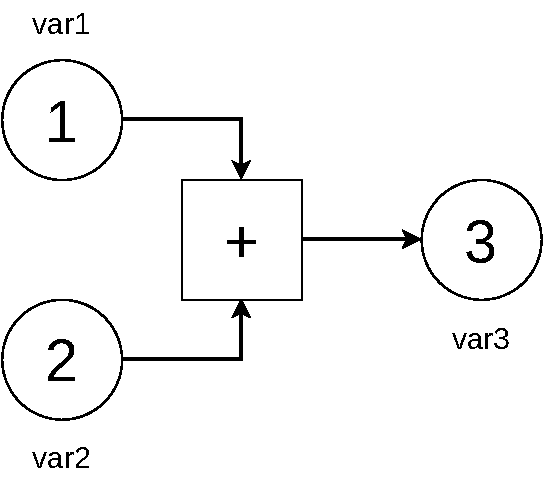
\includegraphics[width=\linewidth]{figures/reactive-example.pdf}
            \caption{Graphical representation of expression dependencies in \Cref{lst:reactive-example}.}
    \end{subfigure}
\end{figure}

\subsection{Evaluation Model}

The evaluation model of a reactive programming language focuses on how changes propagate across a dependency graph of values and computations. From the programmer's perspective, the automatic propagation of changes is a fundamental aspect of reactive programming. Essentially, any alteration in a value should be automatically transmitted to all computations dependent on it. When an event occurs at a source, computations reliant on that event should be notified of the changes, potentially triggering a recomputation.

At the language level, a crucial design decision involves determining who initiates the propagation of changes. This entails deciding whether the source should \textit{push} new data to its dependents (consumers) or if the dependents should \textit{pull} data from the event source (producer). In the pull-based model, the computation that requires a value needs to ``pull'' it from the source. That is, propagation is driven by the demand for new data. In the push-based model, when the source has new data, it pushes the data to its dependent computations. That is, propagation is driven by the availability of new data.

\subsection{Reactive Operators}

The primary advantage offered by libraries furnishing the reactive streams APIs lies in the provision of operators. These operators are essentially functions applicable to a data stream, adept at solving problems related to the processing of reactive streams, encompassing tasks such as filtering, mapping (\Cref{fig:reactive-map}), and aggregating.

Furthermore, these operator functions are intentionally designed to be composable, signifying their capability to be consecutively linked to construct processing pipelines.

\begin{figure}
    \centering
    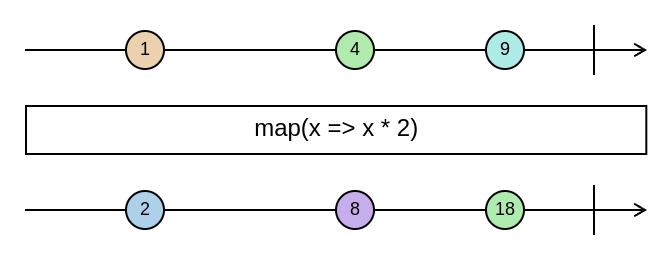
\includegraphics[width=\linewidth]{figures/map-marble.png}
    \caption{Map operator in reactive applications.}
    \label{fig:reactive-map}
\end{figure}

\subsection{Reactive Programming in Kotlin}

Kotlin Flow\footnote{\url{https://kotlinlang.org/docs/flow.html}.} is a part of the Kotlin Coroutines library, introduced to provide a reactive programming model for asynchronous \textit{cold}\footnote{A flow that emits values only when there is an active collector.} and \textit{hot}\footnote{A flow that produces values regardless of whether there are active collectors.} data streams.

A \texttt{Flow} is an asynchronous data stream that sequentially emits values and completes normally or with an exception. Intermediate operators on the flow such as \texttt{map}, \texttt{filter}, \texttt{take} and \texttt{zip} are functions that are applied to the \textit{upstream} flow or flows and return a \textit{downstream} flow where further operators can be applied to. Intermediate operations do not execute any code in the flow and are not suspending functions\footnote{A function that can be paused and resumed at a later time.} themselves. They only set up a chain of operations for future execution and quickly return. This is known as a cold flow property. \textit{Terminal operators} on the flow are either suspending functions such as \texttt{collect}, \texttt{single}, \texttt{reduce} and \texttt{toList} or \texttt{launchIn} operator that starts collection of the flow in the given scope. They are applied to the upstream flow and trigger the execution of all operations. Execution of the flow is also called ``collecting the flow'' and is always performed in a suspending manner without actual blocking. Terminal operators complete normally or exceptionally depending on the successful or failed execution of all the flow operations in the upstream.

By default, flows are \textit{sequential} and all flow operations are executed sequentially in the same coroutine\footnote{A concurrency design pattern that allows to write asynchronous, non-blocking code in a sequential style.}, with an exception for a few operations specifically designed to introduce concurrency into flow execution such as \texttt{buffer} and \texttt{flatMapMerge}.

The \texttt{Flow} interface does not carry information on whether a flow is a cold stream that can be collected repeatedly and triggers execution of the same code every time it is collected, or if it is a hot stream that emits different values from the same running source on each collection. Usually flows represent cold streams, but there is a \texttt{SharedFlow} subtype that represents hot streams. In addition to that, any flow can be turned into a hot one by the \texttt{stateIn} and \texttt{shareIn} operators, or by converting the flow into a hot channel via the \texttt{produceIn} operator.

\begin{figure}[ht!]
    \centering
    \begin{subfigure}[b]{\textwidth}
        \centering
        \lstinputlisting[language=Kotlin,label={lst:flow-example},caption=Kotlin Flow example.]{listings/flow-example.kt}
    \end{subfigure}
    \hfill
    \begin{subfigure}[b]{\textwidth}
        \centering
        \lstinputlisting[label={lst:flow-example-result},caption=Kotlin Flow example result.]{listings/flow-example-result.txt}
    \end{subfigure}
\end{figure}

The example \Cref{lst:flow-example} demonstrates the asynchronous nature of Kotlin Flow and how it allows concurrent execution without blocking the main thread. The \texttt{simple} function creates a flow using the \texttt{flow} builder. Inside the flow, it emits values from 1 to 3 with a delay of one hundred milliseconds between each emission. The delay simulates an operation that takes time, such as network calls or disk I/O. In the \texttt{main} function, a coroutine is launched using \texttt{launch} to run concurrently with the main thread. This coroutine prints messages indicating that it's not blocked and introduces delays between each message. As the flow is collected in the main coroutine, the emitted values are printed and interleaved with the messages from the concurrent coroutine (\Cref{lst:flow-example-result}). This demonstrates that the main thread is not blocked during the execution of the flow, thanks to the asynchronous nature of flows.

\section{Aggregate Computing}
\label{section:aggregate-computing}

\textit{Aggregate computing} is a method for designing intricate coordinations in distributed systems, particularly for \textit{\ac{cas}}~\cite{Ferscha2015}. The approach primarily centers on the notion that understanding system interactions is more straightforward when viewed in the context of information flowing through groups of devices, as opposed to focusing on individual devices and their interactions with peers and the environment~\cite{Viroli2019}.

Aggregate computing is especially suitable for scenarios where the problem at hand involves a network of devices possessing the following characteristics:

\begin{itemize}
    \item \textbf{Openness}, indicating that the surrounding environment where devices operate can undergo unforeseen changes and faults.
    \item \textbf{Large scale}, involving a potentially extensive number of devices or agents that necessitate effective abstractions for coordination.
    \item \textbf{Intrinsic adaptiveness}, signifying the capability to respond to significant events to ensure the overall resilience of the system.
\end{itemize}

Addressing these considerations requires an approach grounded in \textit{self-organization}, where cohesive and resilient coordination behavior arises from localized coordination abstractions. Another objective of aggregate computing is to provide developers with a means to articulate the behavior of distributed systems possessing the aforementioned features in a composable and declarative manner. This facilitates better scalability in dealing with the intricacies of the domain.

Aggregate computing builds upon the principles of \textit{\ac{fc}} (\Cref{subsection:field-calculus}) but adds abstraction layers to address scalability and resilience challenges (\Cref{fig:aggregate-abstraction-layers}). These layers hide the complexity of distributed coordination and support efficient system engineering. The methodology ensures simplicity and transparency in module composition, tailoring coordination mechanisms to different subsystems based on varying requirements. Additionally, it abstracts away intricate implementation details, enabling programmers to focus on high-level system design rather than low-level intricacies. The introduction of ``\textit{resilient coordination operators}'' is fundamental in concealing complexity and ensuring system robustness. By providing standardized ways to handle failures and adapt to changing conditions, these operators contribute to the overall efficiency and reliability of distributed coordination systems.

\begin{figure}
    \centering
    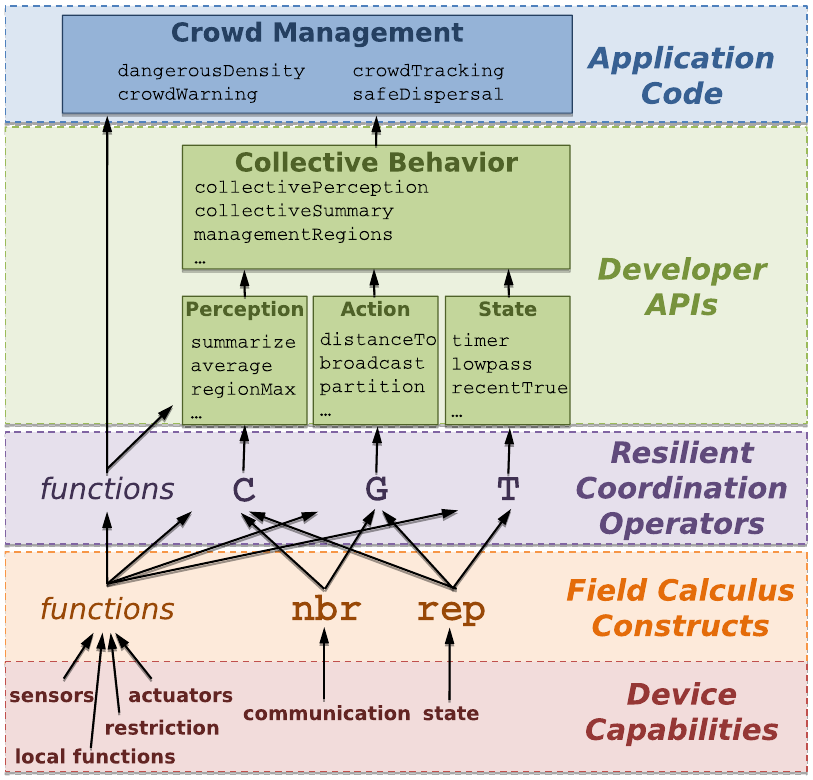
\includegraphics[width=.8\linewidth]{figures/aggregate-programming-abstraction-layers.png}
    \caption{Aggregate programming abstraction layers. The software and hardware capabilities of particular devices are used to implement aggregate-level field
    calculus constructs. These constructs are used to implement a limited set of building-block coordination operations with provable resilience properties,
    which are then wrapped and combined to produce a user-friendly API for developing situated \ac{IoT} systems.}
    \label{fig:aggregate-abstraction-layers}
\end{figure}

\subsection{Abstractions}
\label{subsection:abstractions}

Aggregate computing models a distributed system as a set $\mathcal{D}$ of devices, ranged over by $\delta$. On top of that, a reflexive~\footnote{Each device is a neighbor of itself.} \textit{neighboring relation} indicates the devices with which one can communicate (which is application-dependent and can be used to describe logical or physical proximity). In addition, each device has a set of \textit{sensors} that enable the perception of the environment.

The primary abstraction introduced by aggregate computing is the \textit{computational field} (or simply \textit{field}), which is a function $\phi: \mathcal{D} \mapsto \mathcal{L}$ mapping each device $\delta \in \mathcal{D}$ to a local value $l \in \mathcal{L}$~\cite{Viroli2018}.
%
A \textit{field evolution} is a dynamically changing field, and a \textit{field computation} takes field evolutions as inputs and produces field evolutions as outputs.
%
These outputs are defined in such a way that they change tracking input changes.

The key idea of aggregate computing is that any field computation (\textit{global interpretation}) can be mapped to a \textit{single-device behavior} that is iteratively executed by all the devices in the network (\textit{local interpretation}).
%
Each iteration executed by a device is called a \textit{computation round} and can be subdivided into three steps:
%
\begin{itemize}
    \item \textbf{sense}: the device gathers information coming from its neighbors and local sensors, which are collected to create its \textit{local context} (or \textit{local state}) for the current round;
    \item \textbf{eval}: the computation defined by the behavior is evaluated against the local context, producing an \textit{export};
    \item \textbf{broadcast}: the export is broadcasted to all the device's neighbors, which in turn collect and use this information in their future rounds.
\end{itemize}

\subsection{Field Calculus}
\label{subsection:field-calculus}

Aggregate computing builds from a foundation of the field calculus, a functional programming model for the specification and composition of collective behaviors with formally equivalent local and aggregate semantics.

The concept of field calculus was introduced in~\cite{Viroli2013} as a fundamental core calculus designed to encapsulate the essential elements found in languages utilizing computational fields. These include functions operating over fields, functional composition involving fields, the progression of fields over time, the creation of fields of values based on neighboring elements, and the limitation of a field computation to a specific sub-region within the network. While its syntax, typing, and semantics are deeply discussed in~\cite{Viroli2019} and are omitted here for simplicity, a brief description of its elements is presented below and in \Cref{fig:field-calculus-syntax}:

\begin{itemize}
    \item a \textit{field calculus program} $\texttt{P}$ consists of a sequence of \textit{function declarations} $\bar{\texttt{F}}$ followed by the \textit{main expression} $\texttt{e}$;
    \item an expression $\texttt{e}$ can be:
          \begin{itemize}
              \item a \textit{variable} $\texttt{x}$, e.g., a function parameter;
              \item a \textit{local value} $l$, such as a boolean, number, string, pair, tuple, etc;
              \item a \textit{neighboring field value} $\phi$, e.g., a map of
                    neighbors to the distances to those neighbors;
              \item a \textit{function call} $\texttt{f}(\bar{\texttt{e}})$ to a \textit{user-declared function} or a \textit{built-in function}, such
                    as a mathematical or logical operator, a data structure operation, or a function returning the value of a sensor;
              \item a \textit{branching expression} $\texttt{if} (\texttt{e}_1)\{\texttt{e}_2\}\{\texttt{e}_3\}$ which splits computation into isolated sub-regions, resulting in $\texttt{e}_2$ where and when $\texttt{e}_1$ evaluates to true, and in $\texttt{e}_3$ otherwise;
              \item a $\texttt{nbr}(\texttt{e})$ construct, which creates a neighboring field value that maps each neighbor to the latest result of evaluating $\texttt{e}$;
              \item a $\texttt{rep}(\texttt{e}_1)\{(\texttt{x})\Rightarrow \texttt{e}_2\}$ construct, which models state evolution over time.
          \end{itemize}
\end{itemize}

\begin{figure}
    \centering
    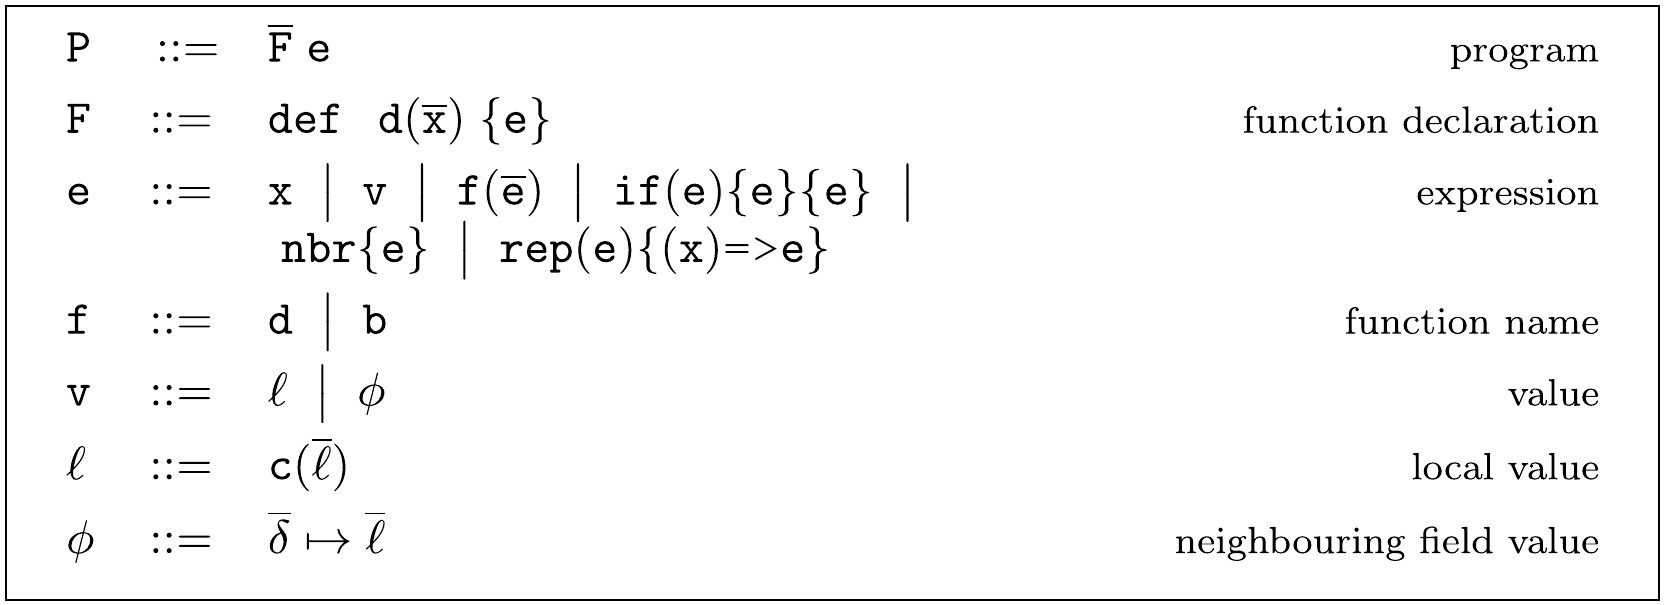
\includegraphics[width=\linewidth]{figures/field-calculus-syntax.jpg}
    \caption{Abstract syntax of the field calculus.}
    \label{fig:field-calculus-syntax}
\end{figure}

To work properly, the semantics of \texttt{nbr} and \texttt{rep} require a way to access, respectively, the last registered state of each neighbor and the last registered output of the device itself. In addition, this process should be made in such a way that different instances of \texttt{rep} and \texttt{nbr} cannot inadvertently ``swap'' their respective value. This process is called \textit{alignment}, and it has the consequence that two branches of an \texttt{if} expression execute in isolation, meaning that two devices that execute different branches cannot communicate with each other inside their branches. In practice, this process is done by carefully constructing the export of an expression as an \textit{evaluation tree} that represents the aggregate computation. The complete semantics of export construction and alignment can be found in~\cite{Viroli2018}.

\subsection{Field Calculus Extensions}

\subsubsection{The Share Operator}

In recent research on the universality of the field calculus, a limitation in the efficiency of information propagation has been identified~\cite{Audrito2018}. This limitation arises from the combination of time evolution and neighbor interaction operators in the original field calculus, resulting in a delay that restricts the speed at which information can be effectively propagated.

The delay stems from the separation between state sharing (\texttt{nbr}) and state updates (\texttt{rep}). Specifically, when information is received through a neighbor operation, it must be retained and remembered through a state update before it can be shared onward during the subsequent execution of the neighbor operation. This process is illustrated in \Cref{fig:handling-state-sharing}.

This delay in information propagation has implications for the efficiency and effectiveness of systems or models built upon the field calculus framework. Researchers may need to explore alternative approaches or optimizations to overcome this limitation and enhance the speed of information dissemination within such systems.

\begin{figure}[ht!]
    \centering
    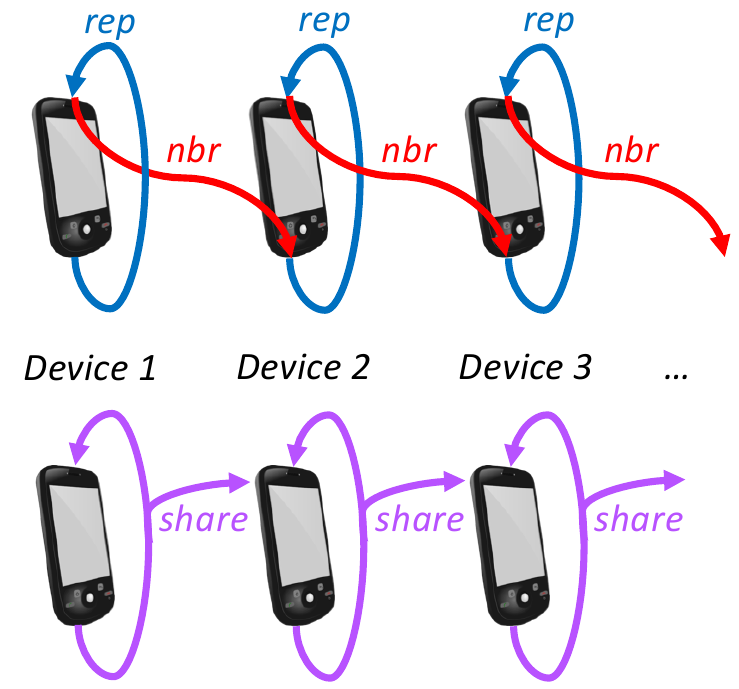
\includegraphics[width=.5\linewidth]{figures/state-sharing.png}
    \caption{Handling state sharing (\texttt{nbr}) and memory (\texttt{rep}) separately injects a delay while information ``loops around'' to where it can be shared (top) while combining state sharing and memory into the new share operator eliminates that delay (bottom).}
    \label{fig:handling-state-sharing}
\end{figure}

In~\cite{Audrito2018} is proposed a solution to the limitation mentioned by introducing the \texttt{share} construct as an extension to the field calculus. This extension is designed to overcome the delay in information propagation by integrating time evolution and neighbor interaction into a single atomic coordination primitive.

The \texttt{share} construct leverages the asynchronous protocol of the field calculus, enabling it to perform several crucial operations simultaneously:

\begin{enumerate}
    \item observation of neighbors' values;
    \item reduction to a single local value;
    \item update of a local variable and sharing of the updated value.
\end{enumerate}

By incorporating these functionalities into a single atomic operation, the \texttt{share} construct enables the immediate sharing of information received from neighbors as soon as it is integrated into the system's state. This eliminates the need to wait for the next computation round, effectively addressing the delay in information propagation identified in the original field calculus framework.

\subsubsection{The XC Language}

Programming distributed systems presents significant challenges, primarily stemming from issues such as concurrency, asynchronous execution, message loss, and device failures. These complexities are particularly pronounced in homogeneous distributed systems, wherein devices are similar and interact with neighboring devices while executing identical programs.

XC is a programming language introduced in~\cite{https://doi.org/10.4230/lipics.ecoop.2022.20}, tailored for the development of homogeneous distributed systems. Within XC, developers craft a singular program that each device executes, facilitating collective emergent behavior. The language's framework abstracts away complexities such as concurrency, asynchronous execution, message loss, and device failures. A minimalist approach is adopted, incorporating a single declarative primitive responsible for communication, state management, and connection oversight (\texttt{exchange}). The alignment mechanism within XC enables developers to abstract over asynchronous execution while preserving composability.

XC features a single communication primitive:

\[ \texttt{exchange($e_i$, $(\underline{n}) \Rightarrow$ return $e_r$ send $e_s$)} \]

which de-sugars to:

\[ \texttt{exchange($e_i$, $(\underline{n}) \Rightarrow$ ($e_r$,$e_s$))} \]

and is evaluated as follows:

\begin{enumerate}
    \item the device computes the local value $l_i$ of $e_i$ (the initial value);
    \item it substitutes variable $\underline{n}$ with the \textit{nvalue} (neighboring value) $\underline{w}$ of messages received from the neighbors for this exchange, using $l_i$ as default. The exchange returns the (neighboring or local) value $v_r$ from the evaluation of $e_r$;
    \item $e_s$ evaluates to a nvalue $\underline{w}_s$ consisting of local values to be sent to neighbor devices $\delta'$, that will use their corresponding $\underline{w}_s$ ($\delta'$) as soon as they wake up and perform their next execution round.
\end{enumerate}

Often, expressions $e_r$ and $e_s$ coincide, hence we provide:

\[ \texttt{exchange($e_i$, $(\underline{n}) \Rightarrow$ retsend $e$)} \]

as a shorthand for:

\[ \texttt{exchange($e_i$, $(\underline{n}) \Rightarrow$ ($e$,$e$))} \]

Another common pattern is to access neighbors' values, which we support via:

\[ \texttt{nbr($e_i$, $e_s$) = exchange($e_i$, $(\underline{n}) \Rightarrow$ return $\underline{n}$ send $e_s$)} \]

In \texttt{nbr($e_i$, $e_s$)}, the value of expression $e_s$ is sent to neighbors, and the values received from them (gathered in $\underline{n}$ together with the default from $e_i$ ) are returned as a nvalue, thus providing a view on neighbors' values of $e_s$. It is crucial for the expressivity of XC that \texttt{exchange} (hence \texttt{nbr}) can send a different value to each neighbor, to allow custom interaction.

\subsection{Reactive and Proactive Models}
\label{subsection:reactive-and-proactive-models}

Aggregate computing emerged as a prominent approach for programming self-organization, with the benefits of formality, abstraction, compositionality, and pragmatism. Formality stems from building the approach over field calculus with well-defined language semantics.

Though conceptually simple, in the round-based model, discussed in~\cite{Viroli2018}, each round of a device is alternated with some sleeping time during which it collects information from neighboring devices. This way of managing computation can be thought of as a \textit{proactive model} since it is the device that decides when computation should occur based on its internal scheduler.

The round-based model could be more efficient because it fully re-evaluates the context and the whole program without tracking change. Though it might be acceptable for predictable patterns of environmental change, this becomes largely suboptimal for highly variable dynamics. Indeed, the round-based approach seems to be a legacy of imperative languages or solutions featuring limited compositionality. Given this motivation, taking inspiration from the functional reactive paradigm, in~\cite{Casadei2023} a \textit{reactive self-organization programming language}, called \ac{frasp}, is proposed. This model enables the decoupling of program logic from its scheduling; the details will be discussed more deeply in \Cref{chap:analysis}.
%! Author = Filippo Vissani
%! Date = 08/02/24
% !TeX root = ../thesis-main.tex

%----------------------------------------------------------------------------------------
\chapter{Analysis}
\label{chap:analysis}
%----------------------------------------------------------------------------------------
\section{State of the Art}

\subsection{Protelis}

Protelis~\cite{Pianini2015} is based on field calculus and is closely related to Proto~\cite{Beal2006}. It inherits spatial computing features from the field calculus, which provides universality, consistency, and self-stabilization properties. However, Protelis improves over Proto by offering a richer API through Java integration, support for code mobility through first-order functions, and a syntax inspired by C-family languages.

The syntax of Protelis (\Cref{fig:protelis-syntax}) is presented in abstract form. It uses meta-variables to represent names of user-defined functions (\texttt{f}), variables and function arguments (\texttt{x}), literal values (l), built-in functions and operators (b), Java method names (\texttt{m}), and aliases of static Java methods (\texttt{\#a}). The syntax employs conventions like comma-separated lists and semi-colon separators for sequences of elements.

Protelis adopts a familiar C- or Java-like syntax, making it more accessible and reducing barriers to adoption. Despite its syntactic similarity to imperative languages, Protelis is purely functional. Programs consist of a sequence of function definitions, followed by a main block of statements. Functions are defined with curly brackets and can contain sequences of statements or expressions. Each statement is an expression to be evaluated (\texttt{e}), possibly in the context of the creation of a new variable (\texttt{let x = e}) or a re-assignment (\texttt{x = e}).

\begin{figure}
    \centering
    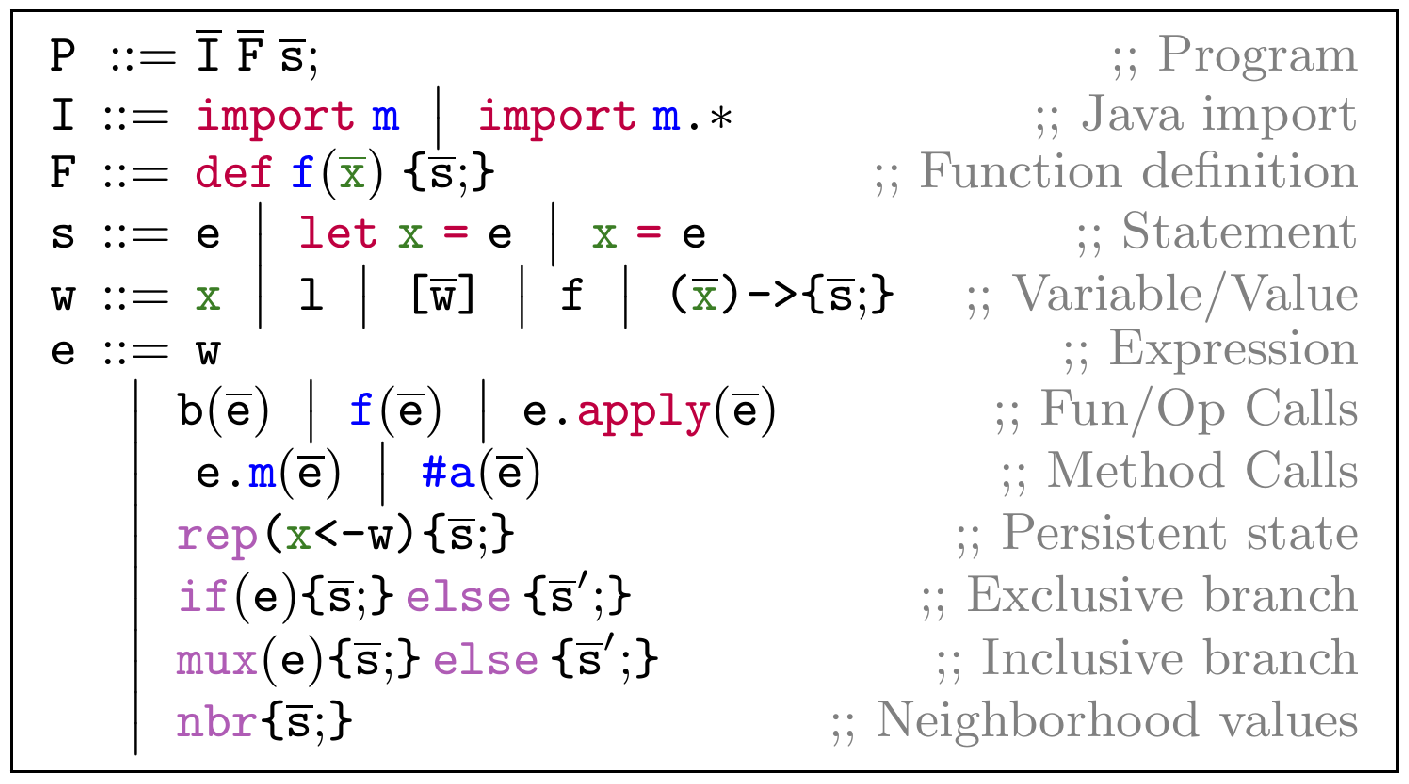
\includegraphics[width=.8\linewidth]{figures/protelis-syntax.png}
    \caption{Protelis abstract syntax}
    \label{fig:protelis-syntax}
\end{figure}

\subsubsection{Example: Rendezvous at a Mass Event}

In large public events, it can be challenging to meet with companions due to crowded areas, inaccessible rendezvous points, or difficulty in accessing cloud-based services.

Utilizing peer-to-peer geometric calculations across a network of devices to compute a \textit{rendezvous}\footnote{A meeting at an agreed time and place.} route is the proposed solution to the problem. The solution is demonstrated in a simulated city center environment (\Cref{fig:protelis-example-map}), using London as an example, with devices distributed randomly across the city streets. Each device has a communication range, and the goal is for two individuals (represented by their devices) to meet at a specific location.

The implementation (\Cref{lst:protelis-example}) involves injecting the environment of the devices with properties representing their owners (e.g., "Alice" and "Bob"). The algorithm measures the distance to one of the participants, creates a potential field, and builds an optimal path from the other participant, descending the distance potential field to reach the first participant at zero distance. The algorithm utilizes two main functions: \texttt{distanceTo} and \texttt{descend}. \texttt{distanceTo} measures the distance to one of the participants. Given a device and a potential field, \texttt{descend} builds a path of devices connecting the device with the source of the potential field. The algorithm elegantly compresses the entire process into a few lines of code, utilizing the \texttt{nbr} operator to exchange required information without explicitly declaring any communication protocol.

As \Cref{fig:protelis-example-map} shows, the simulation rapidly identifies a chain of devices (represented by red dots) that marks a sequence of waypoints for both device owners to walk and meet in the middle. The algorithm dynamically adjusts the path if one of the device owners moves in a different direction, ensuring it continues to recommend the best path for rendezvous.

\lstinputlisting[float,label={lst:protelis-example},caption=Rendezvous implementation in Protelis]{listings/protelis-example.txt}

\begin{figure}
    \centering
    \begin{subfigure}[b]{.49\textwidth}
        \centering
        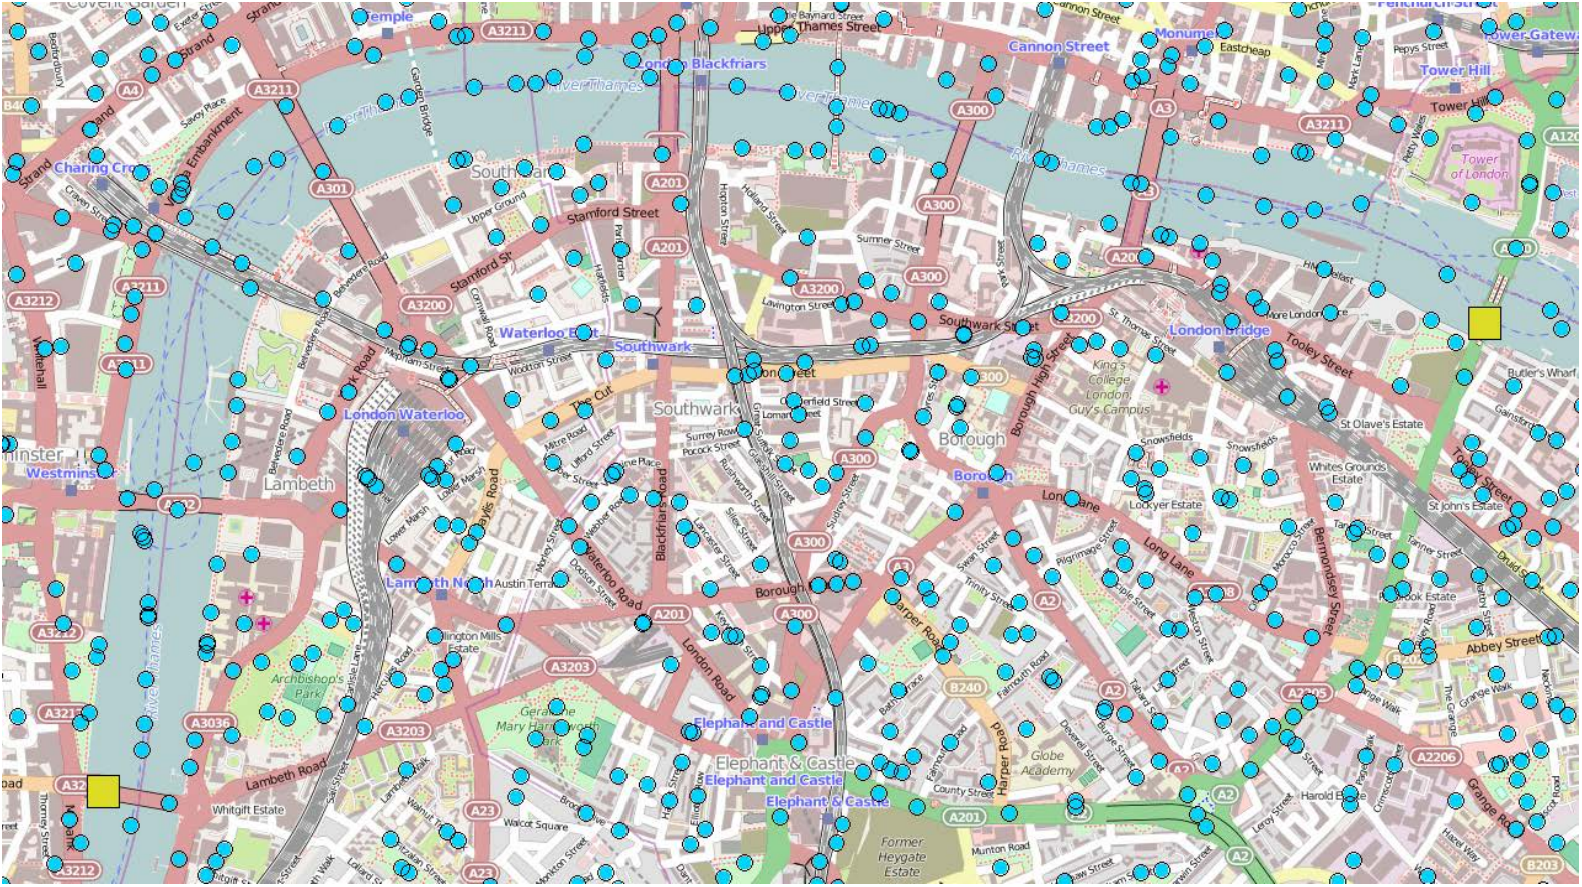
\includegraphics[width=\textwidth]{figures/protelis-example-a.png}
        \caption{Initial configuration.}
        \label{fig:protelis-example-a}
    \end{subfigure}
    \hfill
    \begin{subfigure}[b]{.49\textwidth}
        \centering
        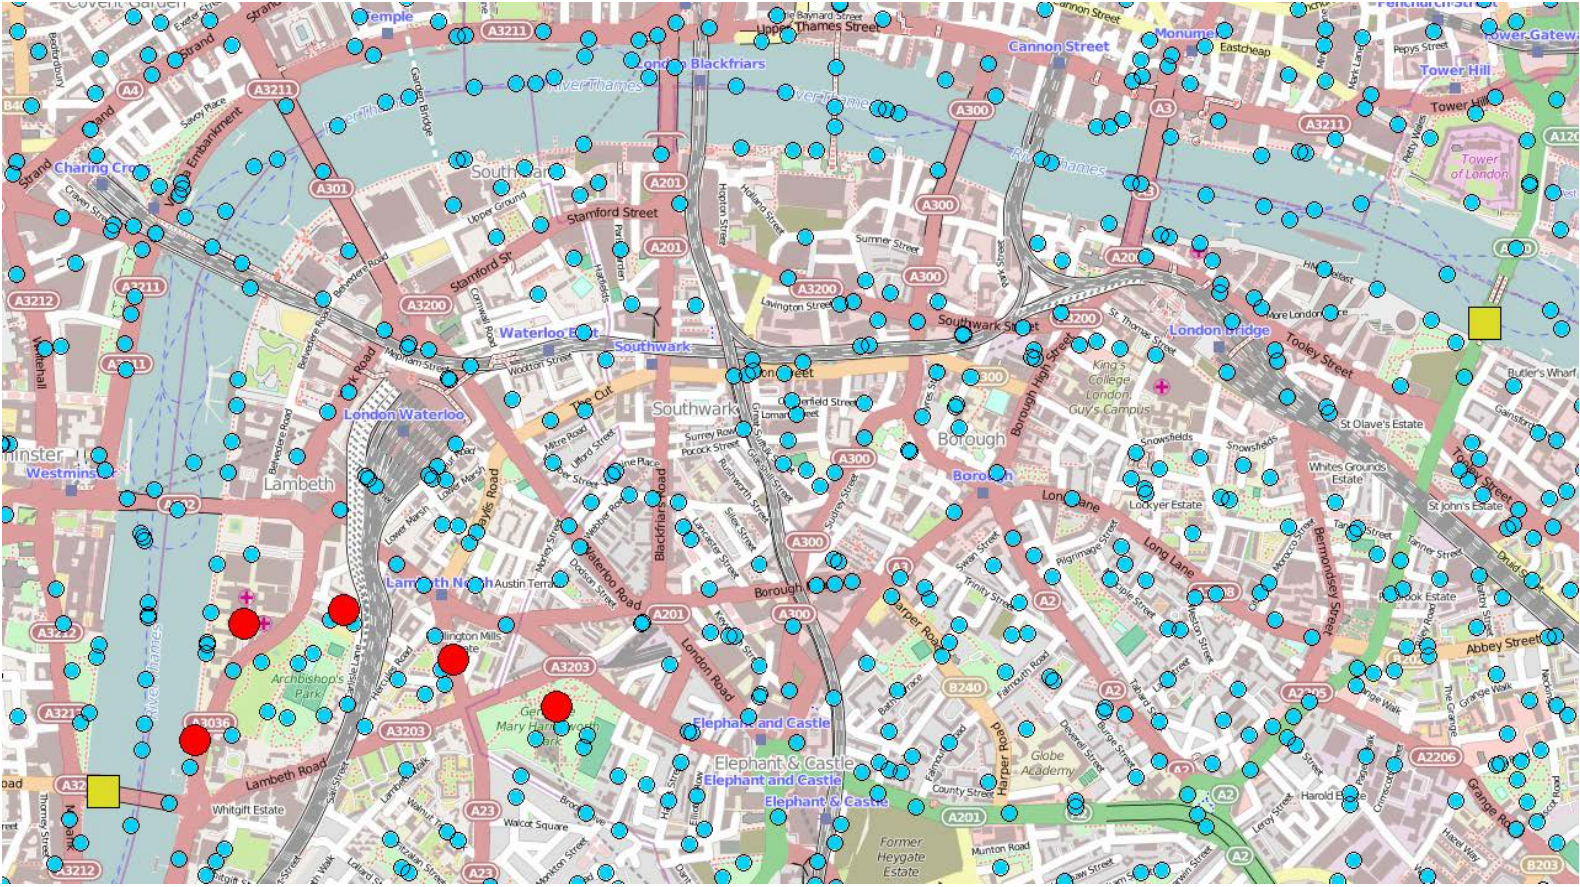
\includegraphics[width=\textwidth]{figures/protelis-example-b.png}
        \caption{Path begins to form.}
        \label{fig:protelis-example-b}
    \end{subfigure}
    \hfill
    \begin{subfigure}[b]{.49\textwidth}
        \centering
        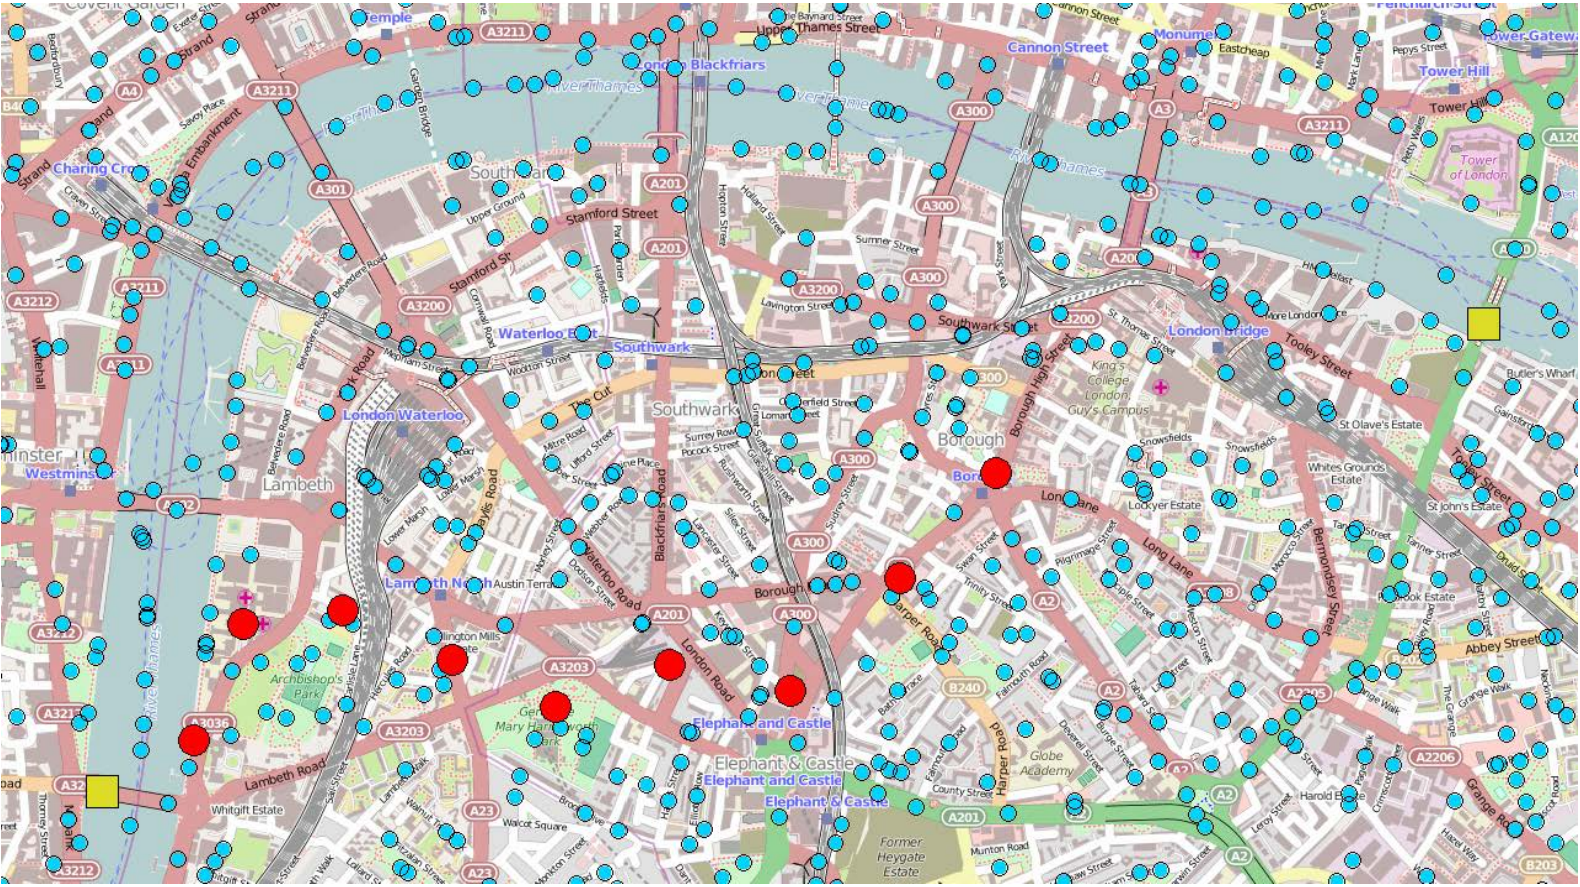
\includegraphics[width=\textwidth]{figures/protelis-example-c.png}
        \caption{Path continues to extend.}
        \label{fig:protelis-example-c}
    \end{subfigure}
    \hfill
    \begin{subfigure}[b]{.49\textwidth}
        \centering
        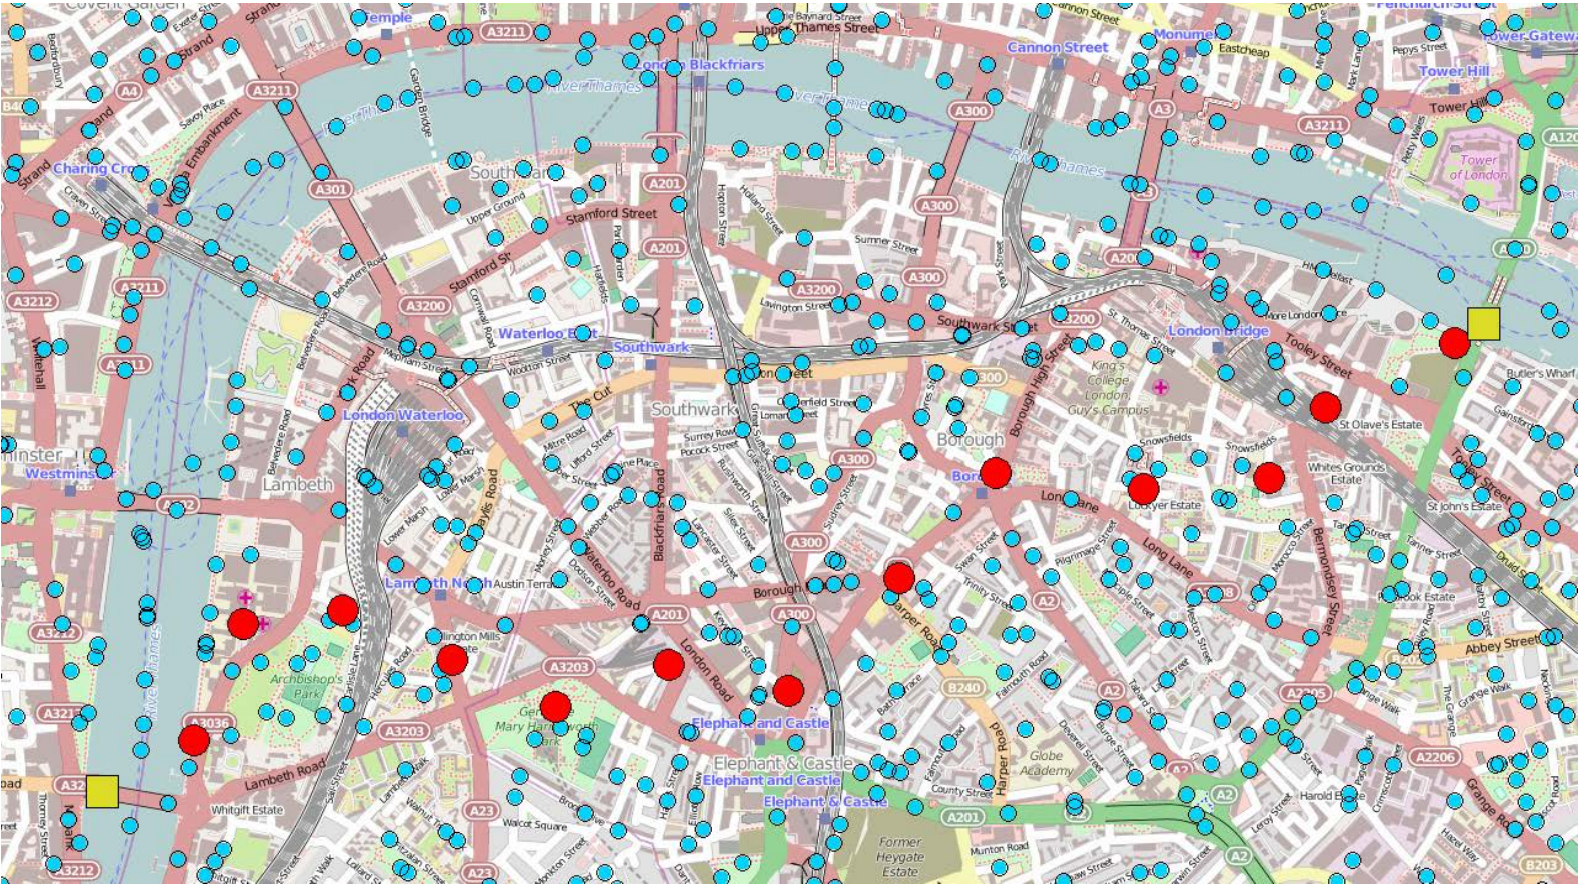
\includegraphics[width=\textwidth]{figures/protelis-example-d.png}
        \caption{Path computation complete.}
        \label{fig:protelis-example-d}
    \end{subfigure}
    \caption{Example of computing a rendezvous route for two people in a crowded urban environment.}
    \label{fig:protelis-example-map}
\end{figure}


\subsection{ScaFi}

ScaFi~\cite{Casadei2022} is a Scala-based library and framework designed for aggregate programming. It facilitates the development of distributed algorithms where computations are performed by individual devices in a network, and the results are aggregated across the network. The core concepts and constructs of ScaFi's API are outlined as follows:

\paragraph{Expression Evaluation}
An expression written using the ScaFi API is evaluated by each device once per computation round.

\paragraph{Fields}
Fields are represented as atomic values without any particular wrapper. They indicate the value of the field at the device performing the computation.

\paragraph{Neighboring Field}
The concept of ``neighboring field" from field calculus is not explicitly represented (not reified). Spatial computation (\texttt{nbr} and \texttt{nbrvar} constructs) is only available inside a special scope provided by the \texttt{foldhood} construct.

\paragraph{Export}
The export for each iteration is constructed by the ScaFi engine. It applies side effects to an internal data structure as the constructs are invoked, thereby constructing the evaluation tree.

\paragraph{Constructs}
The semantics of the constructs defined in ScaFi are described below:
\begin{itemize}
    \item \texttt{rep(init)(f)}: captures state evolution, starting from an \texttt{init} value that is updated each round through \texttt{f};
    \item \texttt{nbr(e)} captures communication, of the value computed from its \texttt{e} expression, with neighbors; it is used only inside the argument \texttt{expr} of \texttt{foldhood(init)(acc)(expr)}, which supports neighborhood data aggregation, through a standard “fold” of functional programming with initial value \texttt{init}, accumulator function \texttt{acc}, and the set of values to fold over obtained by evaluating expr against all neighbors;
    \item \texttt{branch(cond)(th)(el)} captures domain partitioning (space-time branching): essentially, the devices for which \texttt{cond} evaluates to \texttt{true} will run sub-computation \texttt{th}, while the others will run \texttt{el};
    \item \texttt{mid} is a built-in sensor providing the identifier of devices;
    \item \texttt{sense(sensorName)} abstracts access to local sensors;
    \item \texttt{nbrvar(sensorName)} abstracts access to “neighboring sensors” that behave similarly to \texttt{nbr} but are provided by the platform: i.e., such sensors provide a value for each neighbor.
\end{itemize}

\subsubsection{Gradient Implementation in ScaFi}

A \textit{(self-healing) gradient} is a distributed behavior that self-stabilizes, in each device of the distributed system, to a value denoting its minimum distance from the closest source node (for instance, computed by summing the neighbor-to-neighbor distances along the shortest path to the source), adapting to changes in the source set and distances. By following the neighbors of maximum decrease (resp. increase) of the gradient value, i.e., by descending (resp. ascending) the gradient, it is possible to implement efficient hop-by-hop information flows, that can be useful for data propagation and collection.

The implementation of a gradient using ScaFi is presented in \Cref{lst:scafi-gradient}. The following is a brief description of the program:
The gradient value at each node is dynamically evolved using \texttt{rep}. This is necessary to allow a node to share its previous gradient value with neighbors. The default value is \texttt{Double.PositiveInfinity} since by default a node is at an infinite distance from a source (since it may not be reachable in general). The \texttt{mux(c)(th)(el)} evaluates its expression \texttt{th} and \texttt{el} and then uses the Boolean condition \texttt{c} to select either the former (when \texttt{c} is true) or the latter (when \texttt{c} is false).
If a node is a source (i.e., if sensing the Boolean sensor \texttt{source} returns \texttt{true}), then its gradient value is \texttt{0} (by definition).
If a node is not a source, then will take as its gradient value the output of the expression \texttt{minHoodPlus(nbr\{distance\} + nbrRange)}.
\texttt{minHoodPlus(e)} is a variant of \texttt{foldhood} which does not consider the device itself when folding over the neighborhood. Namely, it selects the minimum value among those obtained by evaluating \texttt{e} against the neighbors. The argument of \texttt{minHoodPlus} is \texttt{nbr\{distance\} + nbrRange()}, which amounts to calculating, for each neighbor, the sum of the neighbor's most recent gradient value and the corresponding distance to that neighbor (obtained by neighboring sensor \texttt{nbrRange}, which is \texttt{nbrvar[Double]("nbrRange")}).

\lstinputlisting[float,label={lst:scafi-gradient},language=scala,caption=Implementation of gradient in ScaFi]{listings/scafi-gradient.scala}

\begin{figure}
    \centering
    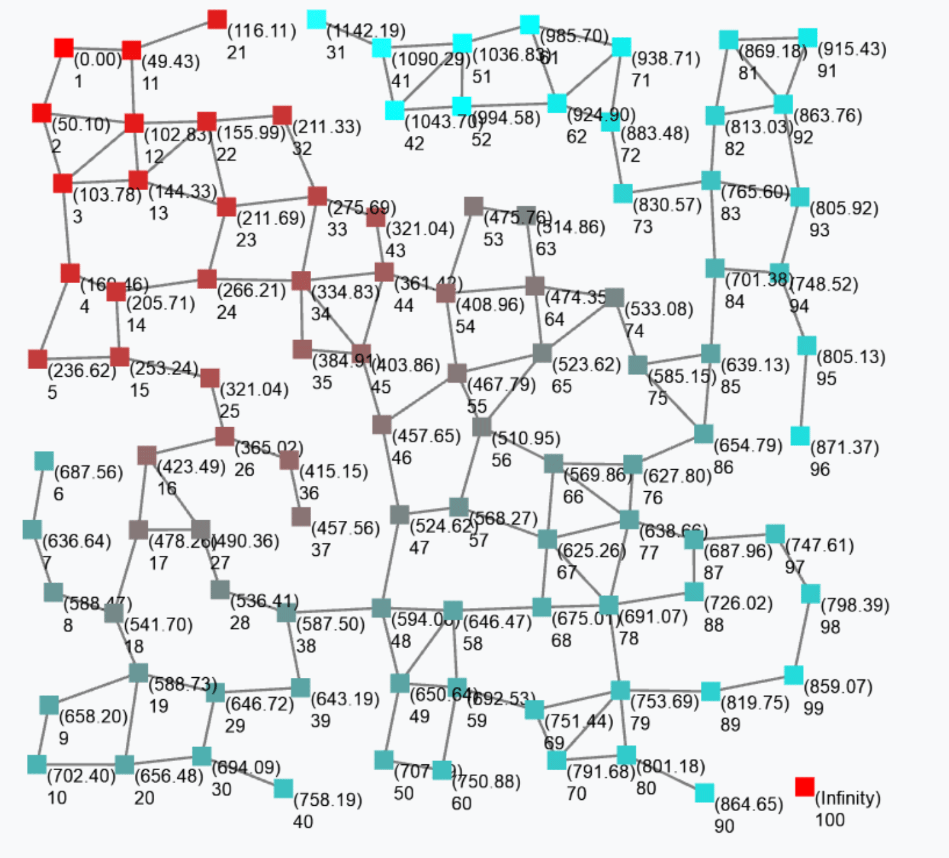
\includegraphics[width=\linewidth]{figures/scafi-gradient.png}
    \caption{A graphical representation of the gradient implementation in ScaFi after stabilization. Each device of the network is labeled with its distance from the source (in parenthesis) and its ID. The source device is the one with ID 1. Note that devices that are not connected to the source are considered to be at an infinite distance from it.}
    \label{fig:scafi-gradient}
\end{figure}

\subsection{FCPP}

FCPP~\cite{Audrito2020} is a C++14 library implementing Field Calculus and providing tools for distributed system simulation.

Its extensible component-based architecture allows customization for diverse application scenarios, such as Internet-of-Things (IoT) deployments, simulations, and self-organizing cloud applications. Users can add components tailored to specific functionalities, enhancing flexibility and applicability. The library incorporates compile-time optimizations and supports parallel execution, enabling efficient simulation of both systems and self-organizing cloud applications. Currently, FCPP focuses on distributed system simulations but already significantly reduces simulation costs, accelerating the development of new distributed algorithms. These features offer a path for a convenient extension to address previously ineffective scenarios:

Existing implementations often have high-performance requirements, unsuitable for resource-constrained microcontrollers. FCPP's lightweight nature makes it well-suited for these systems.

Self-organizing cloud applications necessitate fine-grained parallelism for scalability, and performance improvements directly translate to cost reduction. FCPP's support for parallelism caters to this need.

\subsubsection{Aggregate Program Example with FCPP}

The example function provided in \Cref{lst:fcpp-example} utilizes the Adaptive Bellman-Ford algorithm to estimate distances from devices where the \texttt{source} parameter is \texttt{true}. This function explicitly takes a \texttt{node} object as input, enabling access to its functionalities, including the \texttt{nbr\_dist()} method. This method returns a \texttt{field<double>} representing the estimated distances to neighboring nodes.

The \texttt{call\_point} parameter serves two purposes:

\begin{itemize}
    \item Updating the \texttt{node.stack\_trace} (shared functionality across all aggregate functions, as noted in the first line).
    \item Facilitating the aggregation of function calls (e.g., \texttt{nbr} and \texttt{min\_hood}) by providing an incrementing index.
\end{itemize}

\lstinputlisting[float,label={lst:fcpp-example},language=C++,caption=Implementation Adaptive Bellman Ford algorithm in FCPP]{listings/fcpp-example.cpp}

\subsection{Collektive}

Collektive\footnote{\url{https://github.com/Collektive/collektive}} provides the user with a DSL, implemented in Kotlin, that allows to create aggregate programs transparently. It was designed with the following principles in mind: transparency, minimality and portability.

Transparency refers to the clear and concise information it provides about how the underlying system behaves, such as data processing, storage, and communication between nodes. Transparency helps to reduce complexity, making it easier to understand and maintain large and complex systems.

Collektive is designed with the fewest possible constructs and abstractions while still offering the required functionalities. This reduces the complexity of the system, making it easier to maintain and debug, and lowers the overhead associated with using the DSL, which is particularly important for systems that require high performance and scalability.

Portability refers to its ability to run on various platforms and environments, including different operating systems, cloud platforms, and hardware architectures. This enables systems built with the DSL to be easily deployed and run in different environments, which is crucial for systems requiring deployment in multiple locations or scalability to meet changing demands.

Constructs implemented in Collektive are defined in \Cref{lst:collektive-constructs}, while the semantics are described below:

\begin{itemize}
    \item \texttt{exchange}~\cite{https://doi.org/10.4230/lipics.ecoop.2022.20}: manages the computation of values between neighbors in a specific context. It computes a \texttt{body} function starting from the \texttt{initial} value and the messages received from other neighbors, then sends the results from the evaluation to specific neighbors or everyone, it is contingent upon the origin of the calculated value, whether it was received from a neighbor or if it constituted the initial value. The result of this function is a field with as messages a map with as key the ID of the devices across the network and the result of the computation passed as relative local values.
    \item \texttt{exchanging}: Same behavior of \texttt{exchange} but this function can yield a \texttt{Field} of \texttt{Return} value.
    \item \texttt{repeat}: Iteratively updates the value computing the \texttt{transform} expression at each device using the last computed value or the \texttt{initial}.
    \item \texttt{repeating}: Iteratively updates the value computing the \texttt{transform} expression from a \texttt{YieldingContext} at each device using the last computed value or the \texttt{initial}.
\end{itemize}

\lstinputlisting[float,label={lst:collektive-constructs},language=kotlin,caption=Base constructs implemented in Collektive]{listings/collektive-constructs.kt}

\subsubsection{Example of Gradient in Collektive}

In the \Cref{lst:collektive-gradient}, the implementation of the gradient in Collektive is presented. In this case, a construct is used that is not strictly part of the field calculus but extends it; it is the \texttt{share} construct~\cite{https://doi.org/10.48550/arxiv.1910.02874}. \texttt{share} captures the space-time nature of field computation through observation of neighbors' values, starting from an \texttt{initial} value, it reduces to a single local value given a \texttt{transform} function and updating and sharing to neighbors of a local variable.

\lstinputlisting[float,label={lst:collektive-gradient},language=kotlin,caption=Gradient implementation in Collektive]{listings/collektive-gradient.kt}

\subsection{FRASP}

As said in \Cref{subsection:reactive-and-proactive-models}, aggregate computing makes use of a round-based execution model, that can be defined as proactive. This approach is simple to reason about but limited in terms of flexibility in scheduling and management of sub-activities (and response to contextual changes). In~\cite{Casadei2023} is proposed a reactive self-organization programming approach, called FRASP, that enables the decoupling of the program logic from the scheduling of its sub-activities. This model maintains the same expressiveness and benefits of aggregate programming while enabling significant improvements in terms of scheduling controllability, flexibility in the sensing/actuation model, and execution efficiency.

\subsubsection{Reactive Model}
FRASP is based on the functional reactive programming (FRP) paradigm and considers \textit{continuous time}, $Time$ = $\{ t \in \mathbb{R} \, | \, t \geq 0 \}$. Time-varying values are called \textit{cells} and may be conceptually modeled by generic functions of type $Cell$ $a$: $Time \rightarrow a$. Then, \textit{streams} are discrete-time values and may be modeled by generic functions of type $Stream$ $a$: $[Time] \rightarrow [a]$, namely, mapping a sequence of (increasing) sample times to a sequence of corresponding values. While cells model state, streams model state changes.

\subsubsection{Abstractions and Primitives}

One of the main differences between the proactive and reactive models is that the latter allows the self-organizing collective computation to be expressed as a graph of reactive sub-computations. Each sub-computation is called \textit{flow} and represents it programmatically through type \texttt{Flow[T]}, where \texttt{T} is the type of the output of the wrapped computation. A \texttt{Flow} is essentially a function that takes a \texttt{Context} and returns a cell of \texttt{Export}s, possibly depending on the exports of other \texttt{Flow}s, recursively.

The details of the syntax and semantics of FRASP are discussed in detail in Section III of~\cite{Casadei2023} while in this section they are presented in a simplified manner:

\begin{itemize}
    \item \texttt{constant(e)} returns a constant flow that always evaluates to the argument that has been passed;
    \item \texttt{sensor(name)} returns the flow of values produced by the sensor with the given \texttt{name};
    \item \texttt{mid()} returns the constant flow of the device ID;
    \item \texttt{mux(c)\{t\}\{e\}} is an expression that returns a flow with the same output of flow \texttt{t} when the Boolean flow \texttt{c} is true and the output of flow \texttt{e} when \texttt{c} is false;
    \item \texttt{nbr(f)} handles communication with neighbors in both directions at once, it takes a flow \texttt{f} as a parameter;
    \item \texttt{branch(c)\{t\}\{e\}} evaluates and returns the value of expression \texttt{t} when \texttt{c} evaluates to true. This enables a form of distributed branching, where devices that happen to execute \texttt{t} will not interact with those that executed \texttt{e} (and vice versa);
    \item \texttt{loop(init,ft)} evolves a piece of state (initially, \texttt{init}) by applying function \texttt{ft} mapping the previous state's flow to the next state's flow.
\end{itemize}

\subsubsection{Gradient Implementation in FRASP}

\Cref{lst:frasp-gradient} provides a representation of a gradient in FRASP. The function takes the Boolean \texttt{src} flow as input, denoting whether the executing node is the source of the gradient or not. The external \texttt{loop} is used to progressively evolve the current gradient value \texttt{distance} starting from an infinite value (as, initially, devices do not know whether a source is reachable). Internally to the loop, \texttt{mux} is used to select one of two values: if the node is a source, then its gradient value is \texttt{0} (base case); otherwise, the gradient should be the minimum value among the neighbors' gradient values augmented by the distance (\texttt{nbrRange}) from that very neighbor. Construct \texttt{liftTwice} is used to combine (using the sum: \_+\_) the two flows \texttt{nbrRange} (distances to neighbors) and \texttt{nbr(distance)} (neighbors' gradient values).

\lstinputlisting[label={lst:frasp-gradient},language=scala,caption=Gradient implementation in FRASP]{listings/frasp-gradient.scala}

The reactive dataflow graph in \Cref{fig:gradient-dependencies} corresponds to \Cref{lst:frasp-gradient}. \Cref{fig:gradient-dependencies} provides the local view of the computation for a single node (where the layers denote different semantic kinds of dependencies), whereas \Cref{fig:gradient-dependencies-distributed} shows the distributed dependency graph. The arrows denote dependencies. The dashed arrows denote dependencies based on platform-level scheduling and node interaction; for instance, a red block depends on changes corresponding to neighbors' red blocks and is communicated via message passing.

\begin{figure}
    \centering
    \begin{subfigure}[b]{\textwidth}
        \centering
        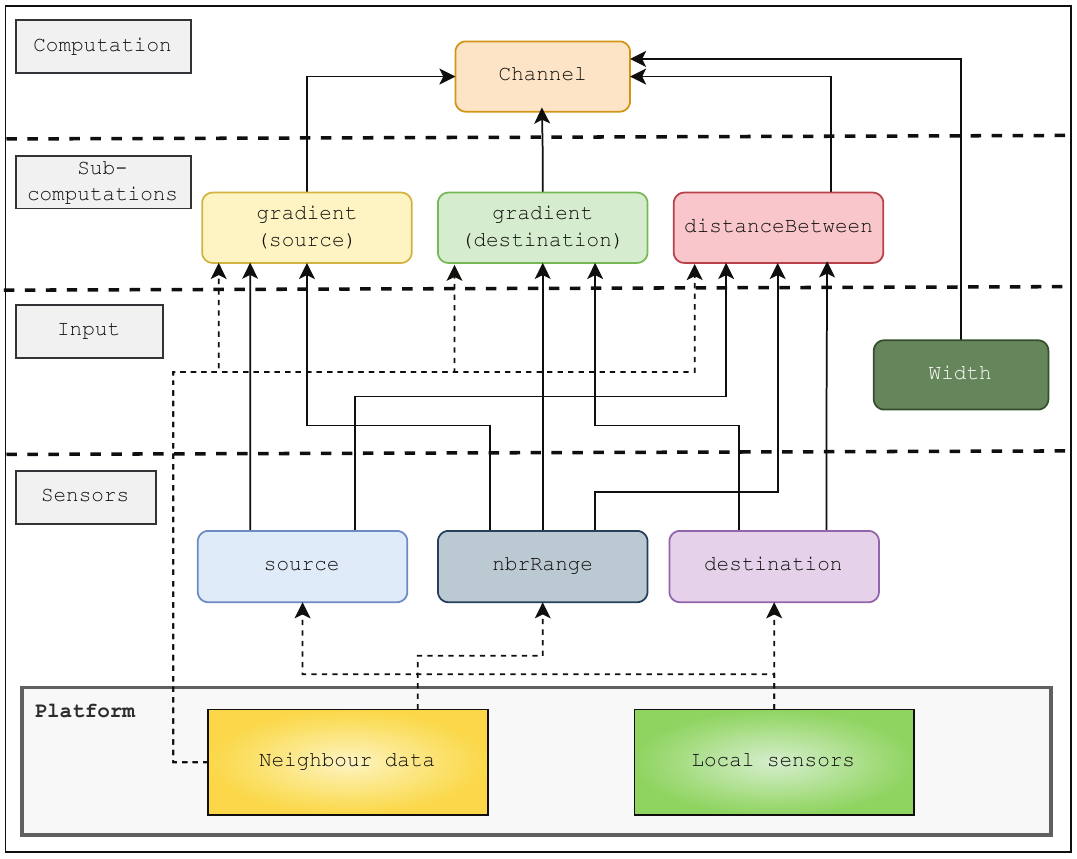
\includegraphics[width=\textwidth]{figures/gradient-dependencies.png}
        \caption{Node view.}
        \label{fig:gradient-dependencies}
    \end{subfigure}
    \hfill
    \begin{subfigure}[b]{\textwidth}
        \centering
        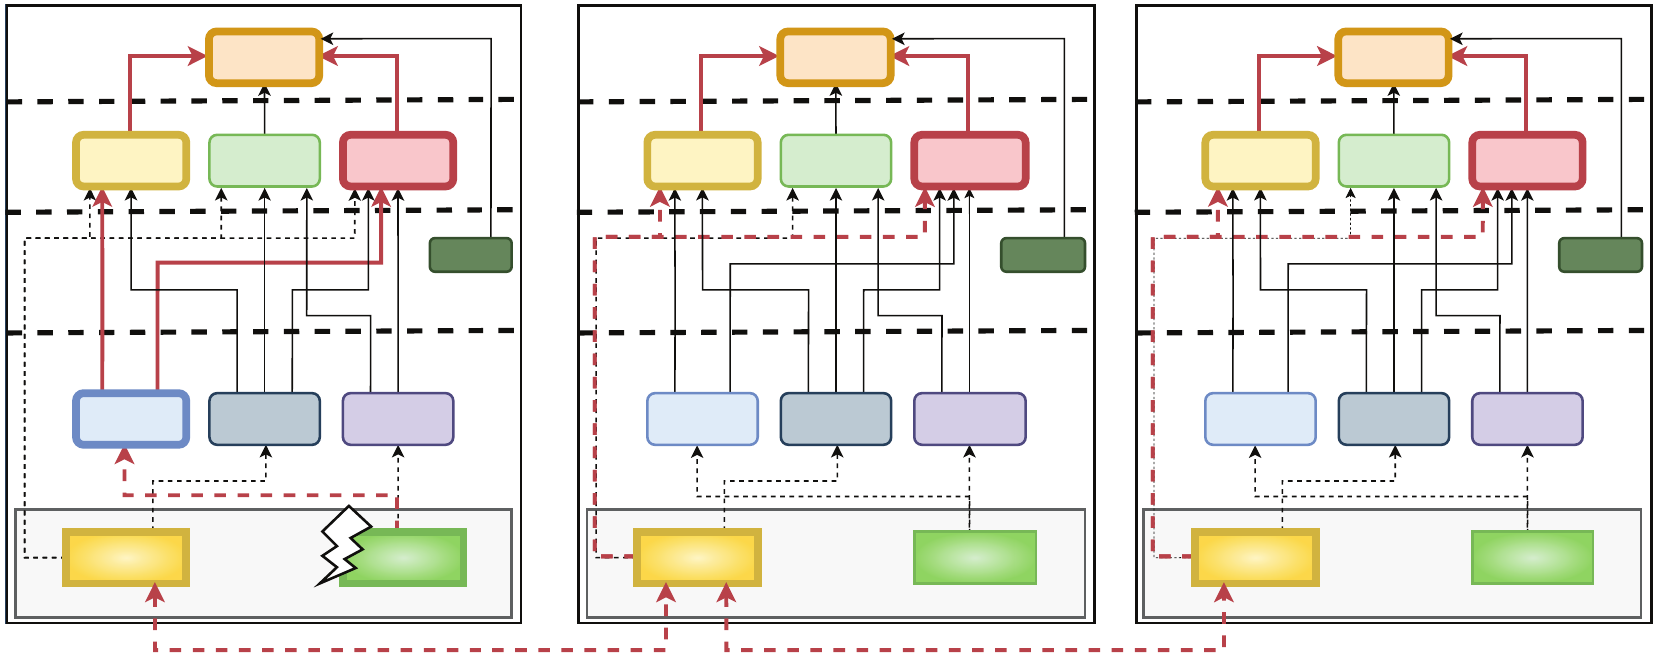
\includegraphics[width=\textwidth]{figures/gradient-dependencies-distributed.png}
        \caption{Distributed view (with neighbor dependencies).}
        \label{fig:gradient-dependencies-distributed}
    \end{subfigure}
    \caption{Dependencies between sub-computations in gradient program (\Cref{lst:frasp-gradient})}
\end{figure}

\section{Design of FRASP}

% talk about constructs and semantics

\section{Design of Collektive}

% talk about constructs and semantics

\section{Integration of FRASP in Collektive}
%! Author = Filippo Vissani
%! Date = 08/02/24
% !TeX root = ../thesis-main.tex

%----------------------------------------------------------------------------------------
\chapter{Design}
\label{chap:design}
%----------------------------------------------------------------------------------------

This chapter delves into the design of a reactive extension for the Collektive framework. Collektive enables the execution of aggregate computations across distributed devices. This chapter introduces two novel models that incorporate reactive principles into Collektive's design.

The chapter begins by providing an overview of the current Collektive architecture. It then outlines the proposed reactive architecture, highlighting the introduced components and their functionalities (\Cref{section:architecture}).

Following the architectural overview, the chapter dives into the detailed design of two reactive models proposed (\Cref{section:detailed-design}).

\section{Architecture}
\label{section:architecture}

As mentioned in \Cref{subsection:collektive-architecture}, Collektive consists of three main modules:

\begin{itemize}
    \item \texttt{dsl}
    \item \texttt{compiler-plugin}
    \item \texttt{alchemist-incarnation-collektive}
\end{itemize}

\texttt{alchemist-incarnation-collektive} is responsible for enabling the integration of Collektive simulations into Alchemist. The \texttt{compiler-plugin} takes care of visiting the abstract syntax tree of the aggregate expression and modifying the function call stack to correctly align the devices that execute the aggregate program. The \texttt{dsl} module defines the following components:
\begin{itemize}
    \item \texttt{aggregate}: deals with defining the context related to a device, the semantics of aggregate constructs, and the data structures necessary for path definition and device alignment;
    \item \texttt{field}: Contains the definition of computational field and the related functionalities for manipulating the latter;
    \item \texttt{state}: defines the association between the paths and the results of their evaluations;
    \item \texttt{path}: Defines the data structures necessary to represent the abstract syntax tree relating to the aggregate expression;
    \item \texttt{networking}: defines the data structures necessary for distributed device communication.
\end{itemize}

Given the solutions proposed in \Cref{subsection:integration-solutions-identified}, in both cases, it is necessary to review some of the entities present in Collektive so that it is possible to detect and react to their changes. Regardless of the detailed solution chosen, given that the Collektive design allows it, it is possible to introduce the necessary functionalities as an extension of the current ones. The proposed architecture is shown in \Cref{fig:collektive-prm-architecture}, the components in gray are part of the current Collektive architecture, and those in orange introduce the entities that enable reactive aggregate programming. The component \texttt{reactive} extends \texttt{aggregate} to introduce a reactive version of the entities described above and \texttt{network} to allow reactive distributed communication between devices. The component \texttt{flow.extensions} is used to simplify some operations for combining and mapping flows. According to this design choice, the other modules in the project (\texttt{compiler-plugin} and \texttt{alchemist-incarnation-collektive}) are not altered; consequently, the reactive model introduced continues to make use of the compiler plugin for the definition of the paths.

\begin{figure}
    \centering
    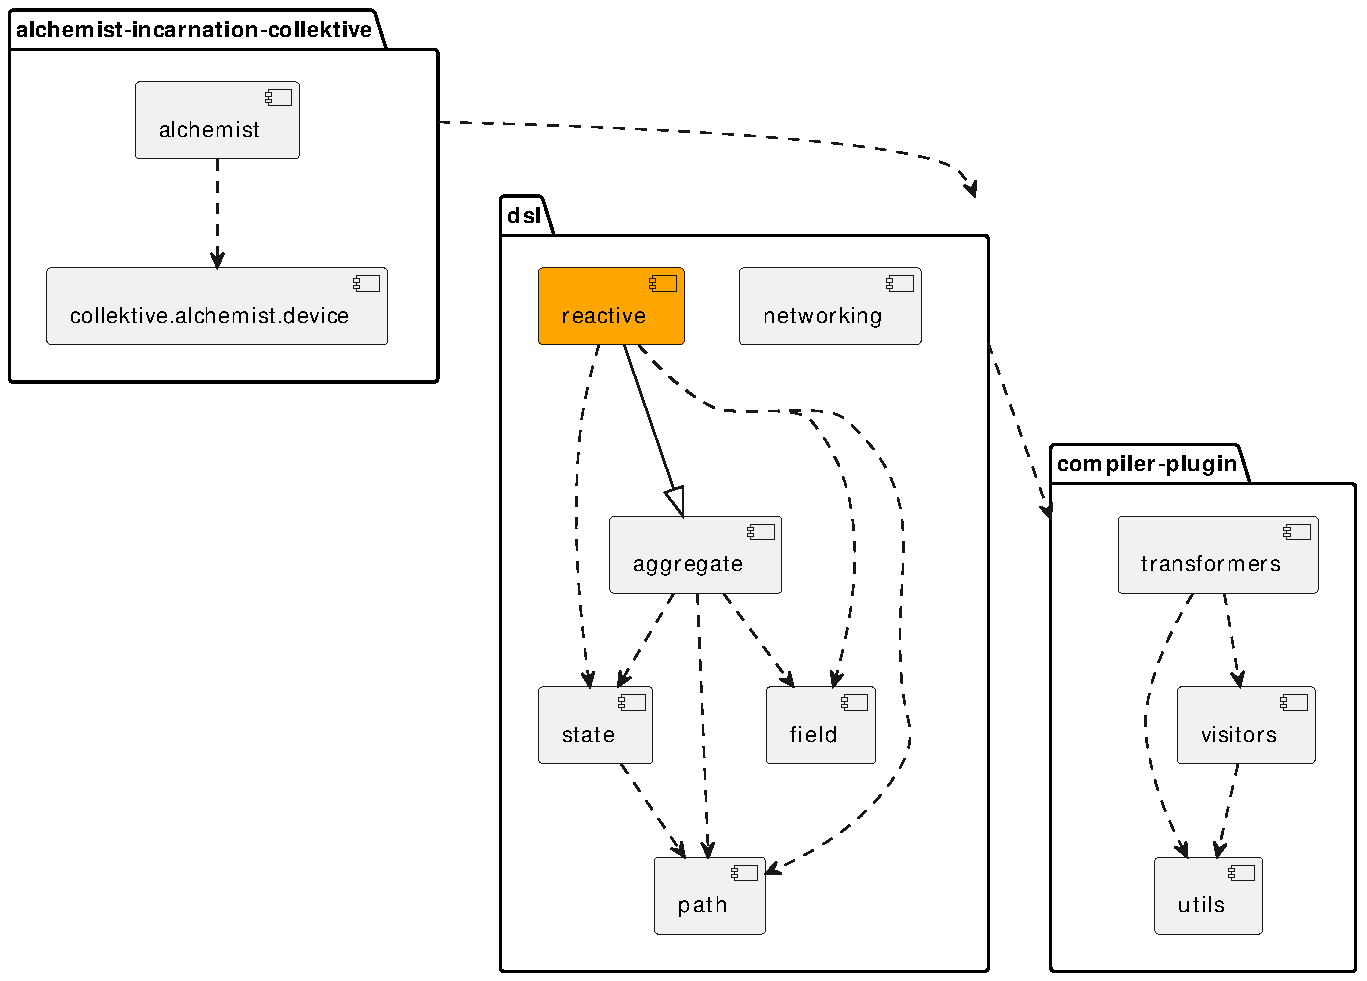
\includegraphics[width=\linewidth]{figures/collektive-prm-architecture.pdf}
    \caption{Architecture of the reactive model proposed. The gray-colored components are part of the original Collektive architecture, while the orange-colored components are used to introduce the reactive paradigm.}
    \label{fig:collektive-prm-architecture}
\end{figure}

\section{Detailed Design}
\label{section:detailed-design}

\subsection{Purely Reactive Model}
\label{subsection:purely-reactive-model}

The detailed design of the \ac{prm} is shown in \Cref{fig:collektive-prm-design}.

Within the \texttt{RCollektive} class, the methods for executing aggregate programs have been augmented to accommodate reactive functionalities. The method \texttt{execute} now takes a \texttt{MutableStateFlow<List<InboundMessage<ID>>>} parameter, enabling the system to react to incoming messages from neighboring devices. Similarly, the \texttt{execute} method now also accepts a \texttt{ReactiveNetwork<ID>} parameter, facilitating reactive communication among devices within the network. These additions signify a departure from the static nature of traditional aggregate computations, allowing for dynamic adjustments based on real-time changes in the environment.

In the \ac{prm}, the concept of expression result (\texttt{RAggregateResult}) is revisited to imbue reactivity. This ensures that the aggregate expression's result is not static but rather dynamic, adapting to alterations in the underlying data or environmental conditions. Moreover, the \texttt{Aggregate} interface undergoes modifications to accommodate reactive versions of aggregate constructs. Parameters within these constructs are bound to \texttt{StateFlow}, enabling reevaluation whenever their inputs experience changes. This reactive paradigm empowers the system to respond dynamically to fluctuations in the environment.

The \texttt{RAggregateContext} class extends the \texttt{Aggregate} interface, providing concrete implementations of reactive aggregate constructs. Additionally, it hosts reactive data structures essential for managing outbound messages and states. Leveraging \texttt{StateFlow} extensions (\texttt{StateFlowExtensions}), this class simplifies the mapping and combining of hot flows, enhancing the efficiency and scalability of the system. By encapsulating reactive functionalities within the \texttt{RAggregateContext}, the system maintains modularity and extensibility, facilitating future enhancements and optimizations.

\subsubsection{Behavioral Characteristics}

The \ac{prm} exhibits distinct behavioral characteristics that distinguish it from traditional static computation approaches:

\begin{itemize}
    \item \textbf{Reactive Computations}: Computation occurs reactively in response to environmental changes, minimizing resource wastage and ensuring optimal responsiveness.
    \item \textbf{Efficient Message Exchange}: Devices only broadcast messages when necessary, reducing unnecessary communication.
    \item \textbf{Selective Reevaluation}: Sub-expressions are reevaluated only when their dependencies change, optimizing computation efficiency and reducing redundant processing.
\end{itemize}

By embodying these characteristics, the \ac{prm} enhances the agility, scalability, and robustness of the Collektive framework, empowering it to effectively handle dynamic and unpredictable environments.

\begin{figure}
    \centering
    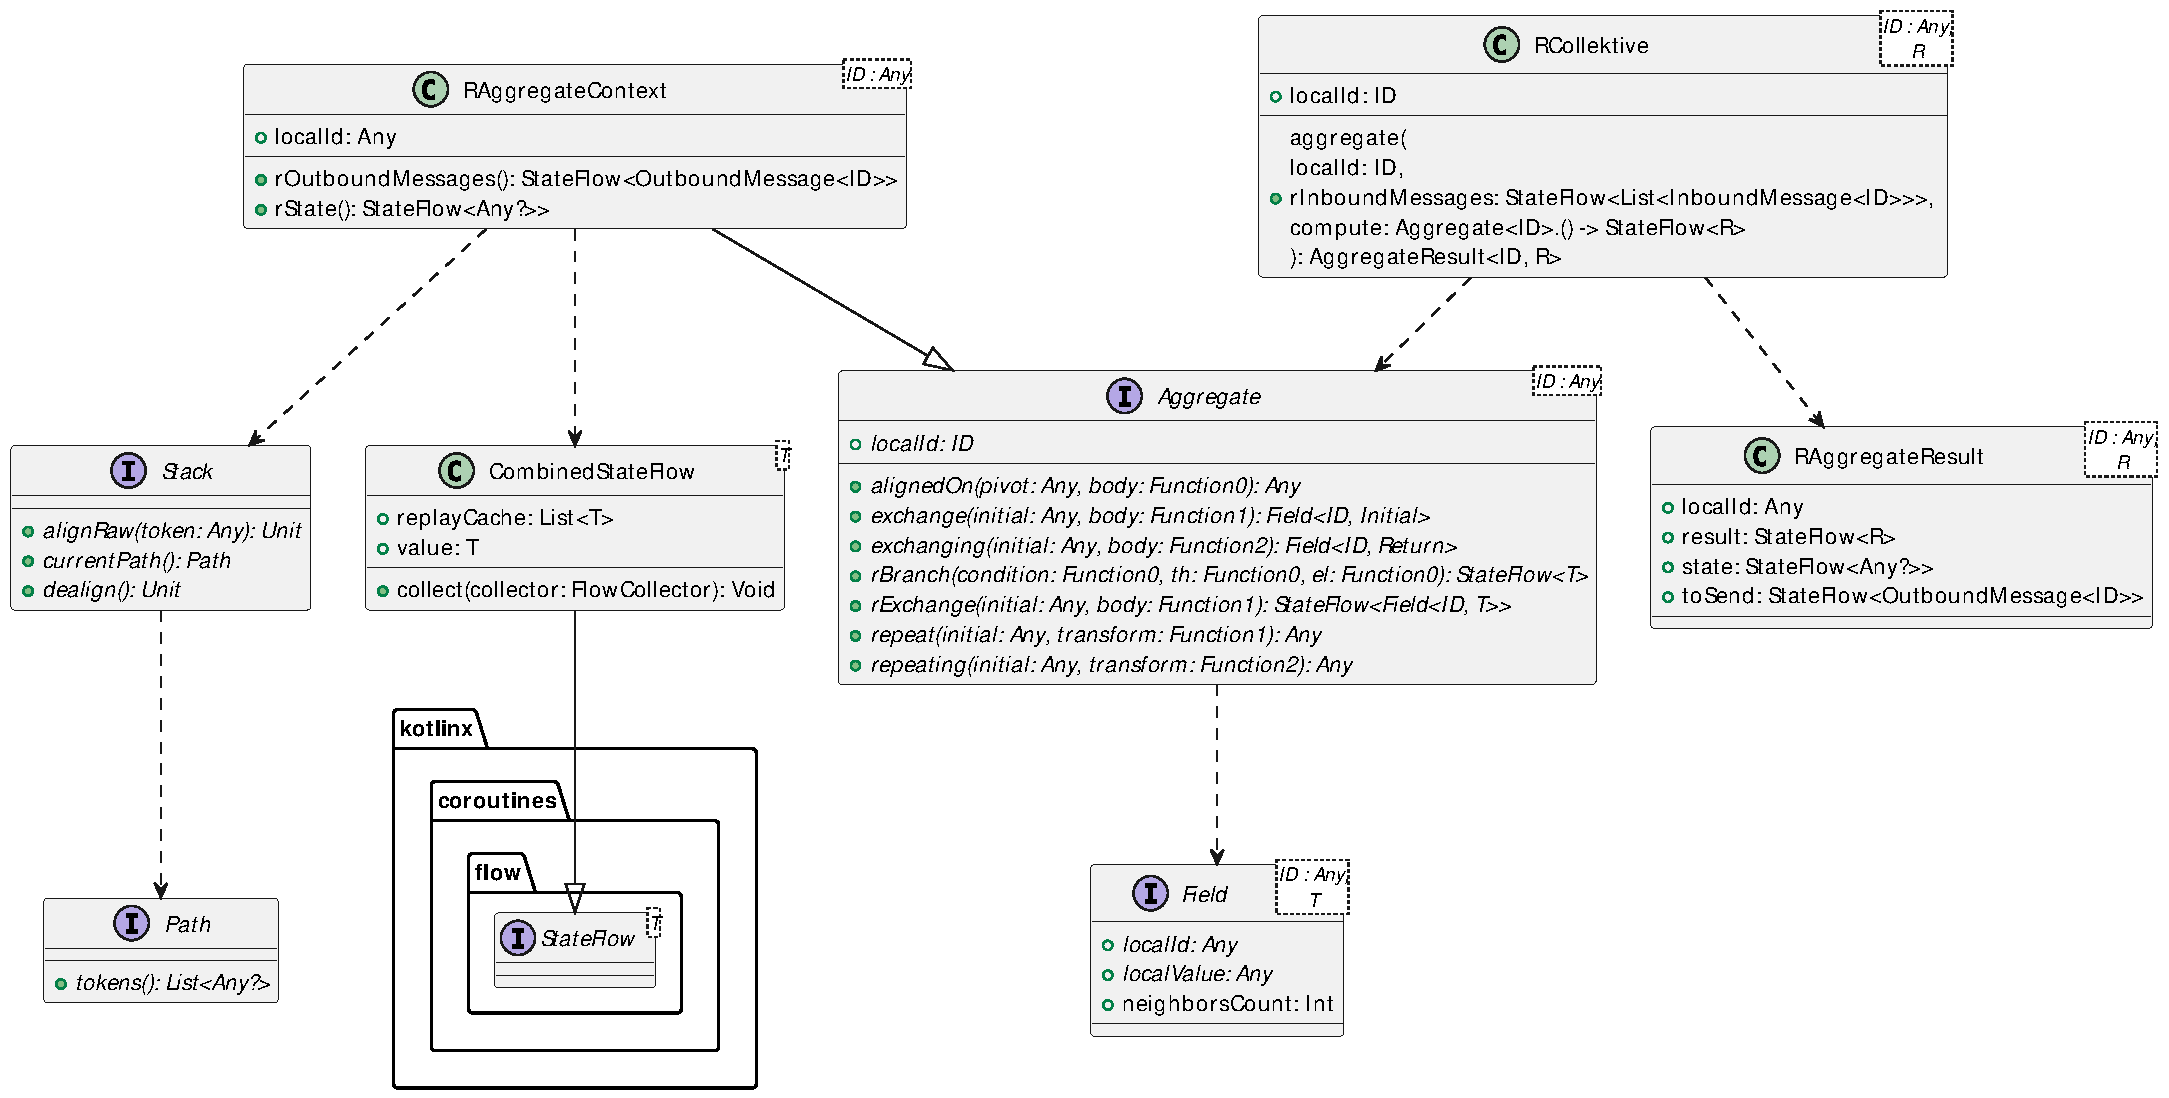
\includegraphics[width=\linewidth]{figures/collektive-prm-design.pdf}
    \caption{Detailed design of the \ac{prm} proposed.}
    \label{fig:collektive-prm-design}
\end{figure}

\subsection{Model with Reactive Messages and Sensors}
The detailed design of the model with reactive messages and sensors is shown in \Cref{fig:collektive-rmsm-design}.

Similar to the \ac{prm}, the \texttt{Collektive} class accommodates two new versions of the \texttt{Aggregate} method to facilitate reactive functionalities. These methods accept either a \texttt{StateFlow<Iterable<InboundMessage<ID>>>} or a \texttt{ReactiveNetwork<ID>} parameter, enabling dynamic adjustment of aggregate computations based on real-time changes in message reception.

In this model, the \texttt{Aggregate} method encompasses the logic necessary for reactive evaluation of the aggregate expression. Unlike the \ac{prm}, where the \texttt{AggregateContext} class handles reactive evaluation, here the evaluation logic is embedded directly within the \texttt{Aggregate} method. Consequently, upon receiving a message from a neighbor, the entire aggregate expression undergoes reevaluation, resulting in a complete round of computation. While maintaining compatibility with the original Collektive \ac{dsl}, this approach sacrifices some performance due to the exhaustive reevaluation process.

\subsubsection{Behavioral Characteristics}

The model with reactive messages and sensors exhibits behavioral characteristics that align with its design principles:

\begin{itemize}
    \item \textbf{Compatibility}: Retains compatibility with the original Collektive \ac{dsl}, ensuring seamless integration with existing codebase and workflows.
    \item \textbf{Simplified Implementation}: Integrates reactive functionalities within the \texttt{Aggregate} method, streamlining the implementation process and reducing complexity.
    \item \textbf{Performance Trade-off}: Sacrifices some performance for compatibility, as the entire aggregate expression undergoes reevaluation upon receiving a message, potentially leading to redundant processing.
\end{itemize}

Despite the performance trade-off, this model provides a pragmatic approach to introducing reactivity into the Collektive framework, catering to scenarios where compatibility and ease of integration are paramount.

In summary, both models offer distinct approaches to incorporating reactive principles into the Collektive framework, each tailored to different use cases and design priorities.

\begin{figure}
    \centering
    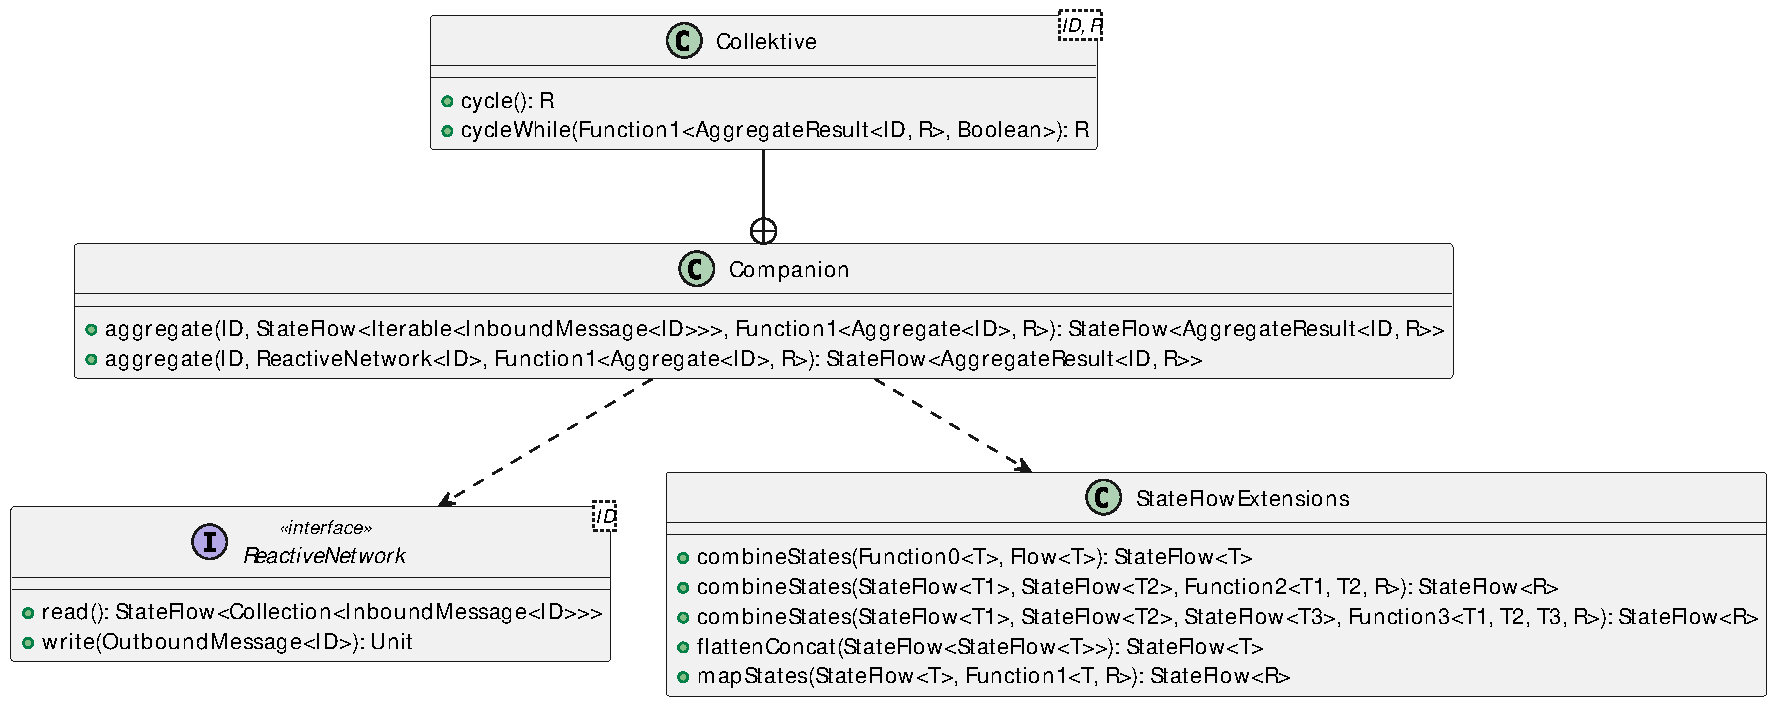
\includegraphics[width=\linewidth]{figures/collektive-rmsm-design.pdf}
    \caption{Detailed design of the model with reactive messages and sensors proposed.}
    \label{fig:collektive-rmsm-design}
\end{figure}

%! Author = Filippo Vissani
%! Date = 08/02/24
% !TeX root = ../thesis-main.tex

%----------------------------------------------------------------------------------------
\chapter{Implementation}
\label{chap:implementation}
%----------------------------------------------------------------------------------------

\section{Purely Reactive Model}

\section{Model with Reactive Messages and Sensors}
%! Author = Filippo Vissani
%! Date = 08/02/24
% !TeX root = ../thesis-main.tex

%----------------------------------------------------------------------------------------
\chapter{Validation}
\label{chap:evaluation}
%----------------------------------------------------------------------------------------

This chapter delves into the evaluation of the reactive extensions introduced into the Collektive framework. The chapter is divided into two main sections:

\begin{itemize}
    \item \Cref{section:testing} details the unit testing strategy employed to ensure the correctness of the implemented code. It highlights the chosen testing framework, and the testing style adopted.
    \item \Cref{section:analysis-ergonomics-proposed-models} compares the usability of the \ac{dsl} for implementing aggregate programs in the two proposed reactive models. To facilitate the comparison, an example program implementing the ``gradient with obstacles'' scenario is presented in both DSLs. This allows for a concrete side-by-side assessment of the strengths and weaknesses of each model from a usability perspective.
\end{itemize}

\section{Testing}
\label{section:testing}

This section delves into the testing strategies employed, focusing on unit testing methodologies.

The project adopts a rigorous approach to testing, leveraging the Kotest\footnote{\url{https://kotest.io/}.} framework for automated testing in Kotlin. Kotest provides a robust testing environment conducive to comprehensive test suites. Among its testing styles, the project opted for \texttt{StringSpec} due to its straightforward structure, which facilitates a behavior-driven approach to test composition. The most relevant tests within the project are those that verify the behavior of the aggregate constructs.

Unit tests are designed to verify the behavior of the aggregate constructs, ensuring they function as expected across various scenarios. Tests are crafted to cover different aspects of the reactive functionality, ensuring the accurate alignment of devices, the correctness of values exchanged and the correctness of aggregate expressions' results.

An example test case for the \texttt{rExchange} construct is presented in \Cref{lst:rexchange-test} to illustrate the testing approach. The test case encompasses the following steps:

\begin{enumerate}
    \item Definition of the test name and sequential execution within a coroutine.
    \item Definition of the aggregate result based on the execution of the aggregate program in a specific aggregate context.
    \item Launching a concurrent job to execute the simulation.
    \item Introduction of a delay and subsequent cancellation of the job.
    \item Assertion of the expected results against the computed values.
\end{enumerate}

The provided example test serves as a template for testing other reactive constructs, ensuring thorough validation of their behavior.

\lstinputlisting[language=kotlin,label={lst:rexchange-test},caption=Part of the test suite related to the \texttt{rExchange} construct.]{listings/rexchange-test.kt}

\section{Analysis of the Ergonomics of the Proposed Models}
\label{section:analysis-ergonomics-proposed-models}

This section evaluates the usability and effectiveness of the proposed reactive models within the Collektive framework. The evaluation focuses on readability, maintainability, flexibility, and the learning curve associated with each model.

The aggregate program chosen to carry out this evaluation is the gradient with obstacles, which maintains the properties of the classic gradient, but introduces obstacles into the environment. \Cref{fig:gradient-environment-and-execution} shows a graphical representation of what we want to achieve. There are three types of nodes in the environment: sources (green), obstacles (red) and defaults (blue). The objective is to calculate the distance of each node from the nearest source without considering the neighbors who are defined as obstacles. The environment used in this case is a grid with five columns and five rows, where each device is a neighbor of the nearest device in each horizontal and vertical direction. In addition, the device with ID 0 is a source node, while devices with ID 2, 7, and 12 are obstacles.

\begin{figure}[ht!]
    \centering
    \begin{subfigure}[b]{.15\textwidth}
        \centering
        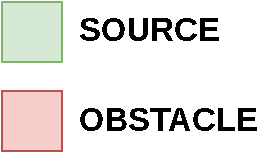
\includegraphics[width=\textwidth]{figures/gradient-environment-legend.pdf}
        \label{fig:gradient-legend}
    \end{subfigure}
    \hfill
    \begin{subfigure}[b]{.49\textwidth}
        \centering
        
\includegraphics[width=\textwidth]{figures/palette-cropped2.png}
        \label{fig:gradient-palette}
    \end{subfigure}
    \hfill
    \begin{subfigure}[b]{.49\textwidth}
        \centering
        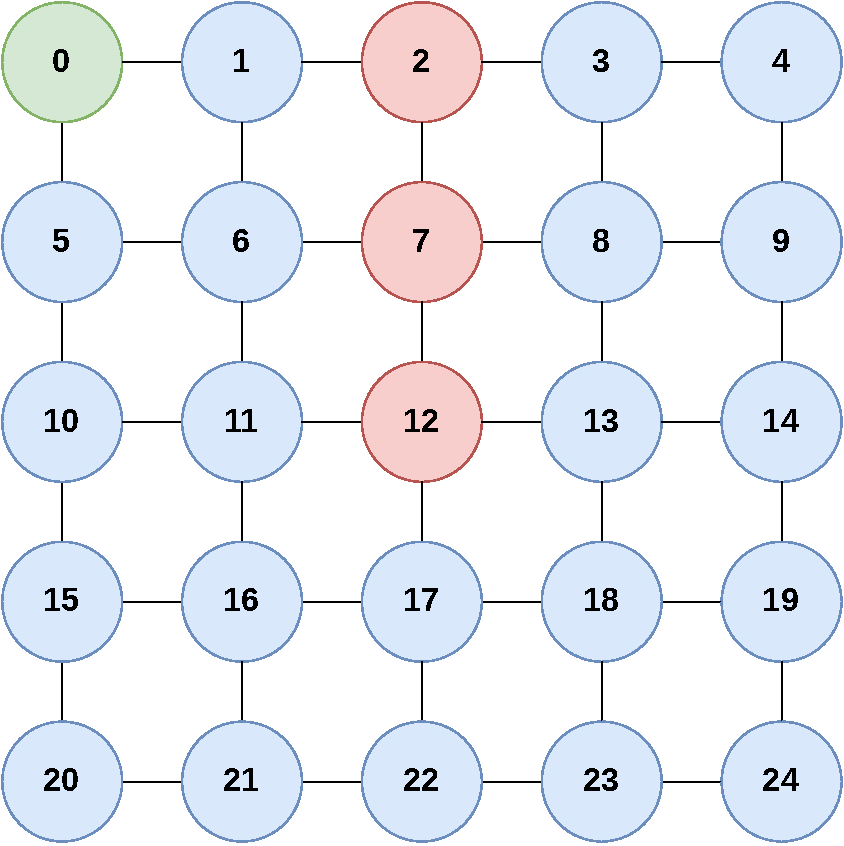
\includegraphics[width=\textwidth]{figures/gradient-environment.pdf}
        \caption{}
        \label{fig:gradient-envronment}
    \end{subfigure}
    \hfill
    \begin{subfigure}[b]{.49\textwidth}
        \centering
        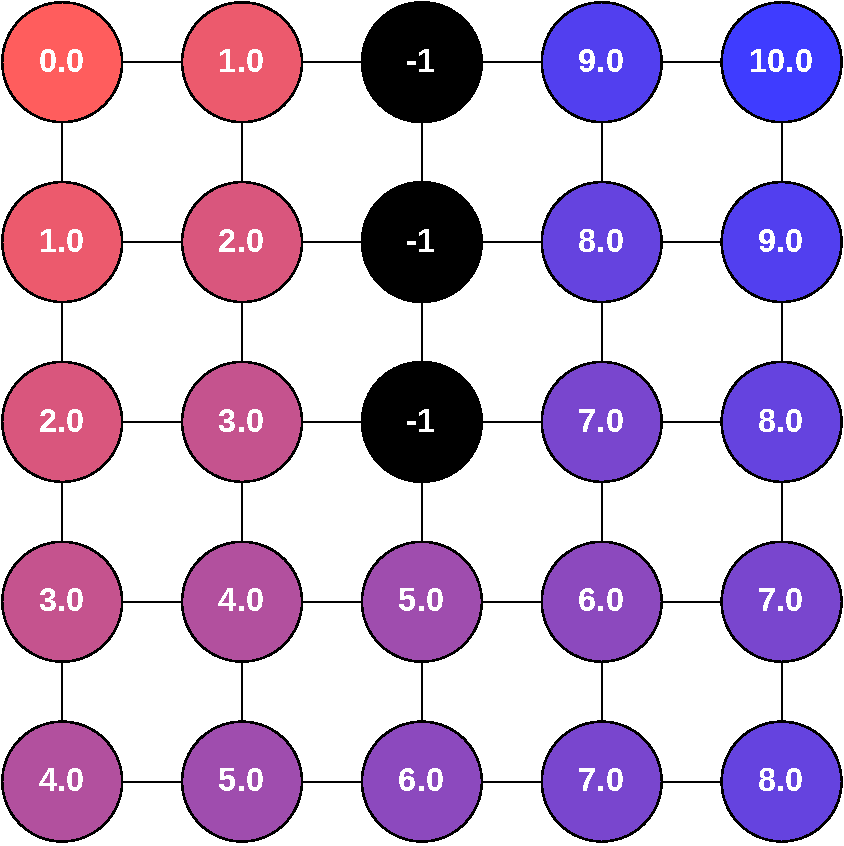
\includegraphics[width=\textwidth]{figures/gradient-environment-execution.pdf}
        \caption{}
        \label{fig:gradient-envronment-execution}
    \end{subfigure}
    \caption{\Cref{fig:gradient-envronment} presents the environment where the gradient with obstacles was executed. The node highlighted in green represents the source, while those in red represent the obstacles. \Cref{fig:gradient-envronment-execution} presents the output field of the gradient with obstacles after stabilization.}
    \label{fig:gradient-environment-and-execution}
\end{figure}

\Cref{lst:gradient-obstacles-prm} and \Cref{lst:gradient-obstacles-rmsm} present the implementation of the gradient with obstacles in the \ac{prm} and in the \ac{rmsm}, respectively. In both cases the node type is defined as \texttt{StateFlow<NodeType>}, allowing to change sources and obstacles at runtime. What changes is how this flow is managed: in the purely reactive case it is used directly within the aggregate constructs, while in the other a specific simulator must be created, which reevaluates the expression as the type of node varies. As regards the use of aggregate constructs within the program, the \ac{rmsm} is equivalent to the proactive model, while in the \ac{prm}, the use of functions for manipulating flows introduces greater complexity.

\lstinputlisting[float,language=kotlin,label={lst:gradient-obstacles-prm},caption=Gradient with obstacles implementation in \ac{prm}.]{listings/gradient-obstacles-prm.kt}

\lstinputlisting[float,language=kotlin,label={lst:gradient-obstacles-rmsm},caption=Gradient with obstacles implementation in \ac{rmsm}.]{listings/gradient-obstacles-rmsm.kt}

The differences between the two implementations are analyzed in detail below:

\begin{enumerate}
    \item Initially, the \texttt{if} (\ac{rmsm}) and \texttt{rBranch} (\ac{prm}) constructs are used to isolate obstacles from the rest of the nodes. Nodes identified as obstacles will return the value -1.0 and will not execute the gradient function. In \ac{rmsm} the condition is verified directly, while in \ac{prm} it is necessary to use the \texttt{mapStates} function to convert the node type into a boolean value. In the \ac{prm}, since the return value is bound to the \texttt{StateFlow} type, to return the value -1.0 (if the condition is true) it is necessary to wrap the latter in a \texttt{MutableStateFlow}. This constraint is not present in the \ac{rmsm}, since the return value does not have to be of type \texttt{StateFlow}.
    \item If the node is not defined as an obstacle, the gradient is executed. The \texttt{share} (\ac{rmsm}) and \texttt{rShare} (\ac{prm}) constructs are used to capture the space-time computation of the gradient. In this case, the way these two constructs are used is very similar.
    \item Internally to \texttt{share} and \texttt{rShare} the \texttt{when} (\ac{rmsm}) and \texttt{rMux} (\ac{prm}) constructs are used, respectively. Both constructs serve to distinguish the source from the rest of the nodes; given a node, if this is identified as the source then the value 0.0 is returned (base case), otherwise, to calculate the return value, the neighbor in which the gradient value is smaller is considered and the distance (1.0) is added. From the two implementations, it appears that the syntax of the \texttt{when} construct is less intricate and more understandable than that used in the \texttt{rMux} construct. Furthermore, within \texttt{rMux} it is necessary to wrap the result in a \texttt{MutableStateFlow} when the condition is true, or use the functions to map flows when the condition is false; these operations are not necessary for the \texttt{when} construct.
\end{enumerate}

\Cref{lst:frasp-gradient2} and \Cref{lst:kotlin-distributed-frp-gradient2} again show the gradient implementations (without obstacles) for FRASP and Kotlin Distributed FRP, respectively. Despite the differences regarding the aggregate constructs, languages (Scala and Kotlin) and the design of the frameworks used, there is some similarity in the four gradient implementations provided.

\lstinputlisting[float,label={lst:frasp-gradient2},language=scala,caption=Gradient implementation in \ac{frasp}.]{listings/frasp-gradient.scala}

\lstinputlisting[float,label={lst:kotlin-distributed-frp-gradient2},language=kotlin,caption=Gradient implementation in Kotlin Distributed FRP.]{listings/kotlin-distributed-frp-gradient.kt}

Based on the results obtained, the following considerations arise:
in the \ac{prm}, the use of \texttt{rShare}, \texttt{rMux}, and \texttt{rBranch} might be less familiar to developers unfamiliar with this specific \ac{dsl}. Understanding the syntax and purpose of these functions requires additional learning. The \ac{rmsm} utilizes familiar syntax like \texttt{share} and conditional statements, potentially making it easier to read and understand for developers with general programming experience.
Composing complex logic using nested functions like \texttt{rMux} and \texttt{rBranch} can lead to nested code structures, potentially impacting maintainability as the codebase grows. In the \ac{rmsm} conditional statements and function calls promote a more linear and explicit flow of logic, potentially improving maintainability.
The \ac{dsl} of the \ac{prm} provides dedicated functions for building reactive constructs, potentially offering more flexibility for complex reactive patterns. While offering less specialized syntax, the \ac{rmsm} can still achieve various reactive behaviors. However, complex reactive patterns might require more verbose code compared to the purely reactive approach.
The \ac{prm} requires learning the specific syntax and semantics of the \ac{dsl} functions, while the \ac{rmsm} leverages familiar programming constructs, potentially reducing the learning curve for developers with general programming experience.

%! Author = Filippo Vissani
%! Date = 08/02/24
% !TeX root = ../thesis-main.tex

%----------------------------------------------------------------------------------------
\chapter{Conclusion}
\label{chap:conclusion}
%----------------------------------------------------------------------------------------

In this thesis, we have explored the feasibility and practicality of implementing reactive aggregate programming in Kotlin for developing artificial self-organizing systems. Our investigation has been guided by the overarching goal of crafting a programming language that enables developers to express macro-level behavior while abstracting away operational details, thus facilitating the self-organizing behavior among a group of agents or devices.

We began by delving into the foundational concepts of functional programming, reactive programming, and aggregate computing, elucidating their relevance and implementations in Kotlin. This served as the bedrock upon which we built our analyses and designs.

Through a critical assessment of existing frameworks such as Protelis, ScaFi, FCPP, Collektive, and \ac{frasp}, we identified key insights and gaps in the current state of the art. Subsequently, we detailed the design of \ac{frasp} and Collektive.

Our investigation into the integration of \ac{frasp} into Collektive unveiled challenges, feasibility considerations, and proposed solutions, underscoring the intricacies involved in harmonizing disparate programming paradigms within a unified framework.

In the design phase, we delineated the architectural and detailed designs of the proposed models, laying the groundwork for their practical implementation. This implementation, divided into sections for the \ac{prm} and the \ac{rmsm}, demonstrated the tangible realization of our theoretical constructs.

In evaluating the proposed models, we subjected them to testing procedures and analyzed their ergonomic aspects, providing valuable insights into their strengths and weaknesses.

In conclusion, our exploration has not only demonstrated the feasibility of reactive aggregate programming in Kotlin but has also contributed to advancing the discourse surrounding programming languages for self-organizing systems. By synthesizing our findings and encapsulating the contributions of this thesis, we pave the way for future research endeavors aimed at further refining and extending the capabilities of programming languages in facilitating the emergence of collective intelligence.

\section{Future Work}

In future work, several areas could be explored to further enhance the capabilities and usability of Collektive:

\paragraph{Support for Real-World Distributed Platforms}

Investigate ways to extend the framework to support deployment and execution on real-world distributed platforms. This could involve optimizations for distributed communication, fault tolerance mechanisms, and integration with existing distributed computing frameworks.

\paragraph{DSL Improvements}

Address the noise introduced in the API of the \ac{prm} due to the necessity of reactive operators to work with flows instead of local values. Research and develop a more streamlined and user-friendly API that abstracts away the complexities of dealing with flows, reducing boilerplate code and improving program transparency.

\paragraph{Timing Configuration Granularity}

Enhance the framework's flexibility in configuring the timing of computations beyond reacting solely to standard events. Explore the possibility of supporting additional strategies for scheduling and rate limiting, such as custom scheduling policies and per-construct configuration options. This could provide developers with finer control over the execution behavior of their self-organizing systems, catering to diverse application requirements and environments.


%----------------------------------------------------------------------------------------
% BIBLIOGRAPHY
%----------------------------------------------------------------------------------------

\backmatter

\nocite{*} % comment this to only show the referenced entries from the .bib file

\bibliographystyle{alpha}
\bibliography{bibliography}

\end{document}